\documentclass[aspectratio=169]{beamer}
 
% ======================= PACOTES =======================
\usepackage[utf8]{inputenc}
\usepackage[T1]{fontenc}
\usepackage[main=brazilian,provide=*]{babel}
\usepackage{amsmath,amssymb,amsthm}
\usepackage{graphicx}
\usepackage{booktabs}
\usepackage{array}
\usepackage{tikz}
\usetikzlibrary{arrows.meta, positioning, shapes.geometric, fit}
 
% ======================= TEMA =======================
\usetheme{Madrid}
\usecolortheme{default}
\definecolor{ufsblue}{RGB}{0,51,102}
\definecolor{ufsblueaccent}{RGB}{40,90,150}
\setbeamercolor{structure}{fg=ufsblue}
\setbeamercolor{palette primary}{bg=ufsblue,fg=white}
\setbeamercolor{palette secondary}{bg=ufsblueaccent,fg=white}
\setbeamercolor{palette tertiary}{bg=ufsblue,fg=white}
\setbeamercolor{title}{fg=ufsblue}
\setbeamercolor{frametitle}{bg=ufsblue,fg=white}
\setbeamertemplate{navigation symbols}{}
\setbeamertemplate{footline}[frame number]
 
% ======================= COMANDO DE PLACEHOLDER DE IMAGEM =======================
\newcommand{\imgph}[2][0.65\textwidth]{%
  \begin{center}
  \setlength{\fboxsep}{0pt}
  \fbox{\begin{minipage}[c][3.6cm][c]{#1}
    \centering
    {\color{gray}\rule{0.9\linewidth}{0pt}}\\
    \textit{\color{gray}[Espaço reservado para imagem]}\\[4pt]
    {\small\color{ufsblue} #2}
  \end{minipage}}
  \end{center}
}
 
% ======================= DADOS DO TRABALHO =======================
% (\title, \subtitle, \author, \institute e \date seguem definidos para
%  alimentar \tableofcontents, o rodapé e metadados do PDF; a capa em si,
%  porém, é construída manualmente logo abaixo para controlar o espaço.)
\title[Análise Topológica em Biologia]{Análise Topológica de Dados Aplicada a Dados de Biologia}
\subtitle{Homologia Persistente na Classificação de Estados Conformacionais da Proteína MBP}
\author[Anthony dos Anjos Marques]{Anthony dos Anjos Marques}
\institute[UFS/DMA]{Universidade Federal de Sergipe}
\date{Julho, 2026}
 
% ======================= INÍCIO DO DOCUMENTO =======================
\begin{document}
 
% ======================= CAPA (layout manual) =======================
% As duas chamadas \includegraphics abaixo são as ÚNICAS que controlam as
% logos da capa. Ajuste apenas a altura (height=...) se elas ficarem
% desproporcionais entre si -- a largura se ajusta automaticamente.
\begin{frame}[plain]
  \begin{tikzpicture}[remember picture, overlay]
    \node[anchor=north west, xshift=0.9cm, yshift=-0.55cm] at (current page.north west)
      {
\includegraphics[height=1.05cm]{Imagens/logo_ufs.png}};
    \node[anchor=north east, xshift=-0.9cm, yshift=-0.55cm] at (current page.north east)
      {
\includegraphics[height=1.05cm]{Imagens/logo_dma.png}};
  \end{tikzpicture}
 
  \vspace{1.4cm}
  \begin{center}
    {\color{ufsblue}\rule{0.42\textwidth}{1pt}}\\[0.28cm]
    {\usebeamercolor[fg]{title}\Large\textbf{Análise Topológica de Dados\\[2pt] Aplicada a Dados de Biologia}}\\[0.25cm]
    {\small\itshape\color{gray!70!black} Homologia Persistente na Classificação de Estados\\ Conformacionais da Proteína MBP}\\[0.25cm]
    {\color{ufsblue}\rule{0.42\textwidth}{0.5pt}}\\[0.32cm]
    {\large\textbf{Anthony dos Anjos Marques}}\\[0.25cm]
    {\footnotesize
      Universidade Federal de Sergipe \;--\; Departamento de Matemática\\
      Bacharelado em Matemática Aplicada e Computacional\\[2pt]
      \textbf{Orientador:} Prof. Dr. Danilo Dias da Silva
    }\\[0.32cm]
    {\footnotesize\color{ufsblue} São Cristóvão -- SE \quad$\vert$\quad Julho, 2026}
  \end{center}
\end{frame}
 

% ======================= SUMÁRIO =======================
\begin{frame}{Sumário}
  \tableofcontents
\end{frame}

% =====================================================================
\section{Introdução}
% =====================================================================

\begin{frame}{Motivação}
  \begin{itemize}
    \item Proteínas não são entidades rígidas: transitam entre estados conformacionais para exercer funções biológicas.
    \item Debate clássico sobre o mecanismo de ligação proteína-ligante:
    \begin{itemize}
      \item \textbf{Encaixe induzido} (\textit{Induced Fit});
      \item \textbf{Seleção conformacional} (\textit{Conformational Selection}).
    \end{itemize}
    \item Métricas geométricas clássicas (RMSD) frequentemente falham em capturar correlações não-lineares e variações dinâmicas globais.
  \end{itemize}
  \centering
  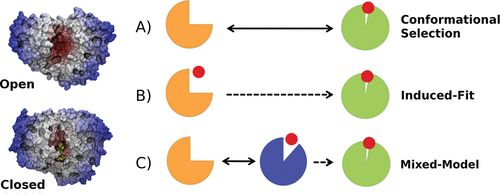
\includegraphics[width=0.6\textwidth]{Imagens/apresentacao_mbp.png}
  % \imgph{Figura 1 -- Modelos de encaixe induzido, seleção conformacional e modelo misto (Bucher et al.)}
\end{frame}

\begin{frame}{A Proteína de Ligação à Maltose (MBP)}
  \begin{columns}[c] % O [c] alinha verticalmente o centro do texto com o centro da imagem
    
    % Coluna da esquerda (Texto)
    \begin{column}{0.6\textwidth}
      \begin{itemize}
        \item Encontrada em \textit{Escherichia coli}; transporta maltodextrinas.
        \item Dois domínios globulares conectados por uma região de dobradiça (\textit{hinge}).
        \item Transita entre dois estados conformacionais:
        \begin{itemize}
          \item \textbf{Apo} -- aberta, livre de ligante;
          \item \textbf{Holo} -- fechada, associada ao ligante (maltose).
        \end{itemize}
      \end{itemize}
    \end{column}
    
    % Coluna da direita (Imagem)
    \begin{column}{0.3\textwidth}
      \centering
      % O width agora é em relação à própria coluna, então usamos \textwidth inteiro
      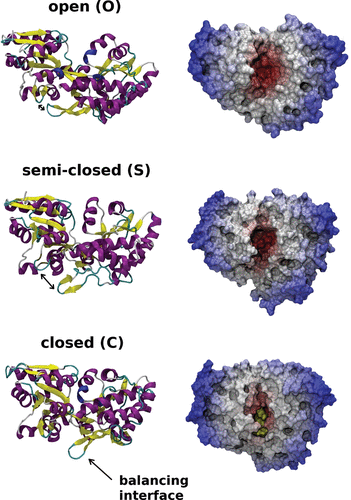
\includegraphics[width=\textwidth]{Imagens/estagios_mbp_3d.png}
    \end{column}
    
  \end{columns}
\end{frame}
\begin{frame}{Objetivo e Estratégia}
  \textbf{Objetivo:} investigar, fundamentar e aplicar a Análise Topológica de Dados (TDA) e a Homologia Persistente na classificação de estados conformacionais da MBP.
  \vspace{0.3cm}
  \begin{center}
  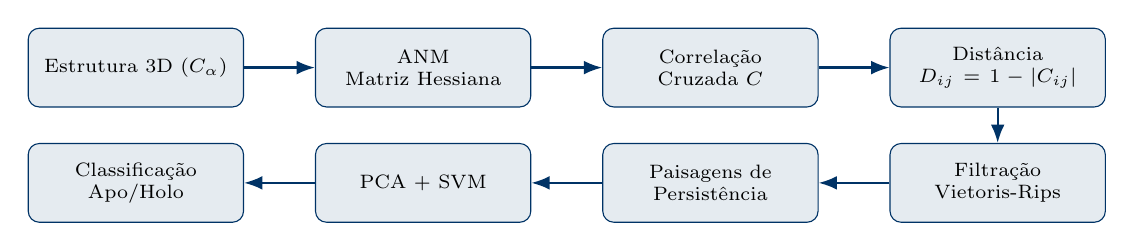
\begin{tikzpicture}[
    node distance=0.45cm and 0.9cm,
    box/.style={draw, rounded corners, fill=ufsblue!10, draw=ufsblue, minimum height=1cm, text width=2.5cm, align=center, font=\scriptsize},
    arr/.style={-{Latex}, thick, ufsblue}
  ]
    \node[box] (a) {Estrutura 3D ($C_\alpha$)};
    \node[box, right=of a] (b) {ANM \\ Matriz Hessiana};
    \node[box, right=of b] (c) {Correlação Cruzada $C$};
    \node[box, right=of c] (d) {Distância $D_{ij}=1-|C_{ij}|$};
    \node[box, below=of d] (e) {Filtração Vietoris-Rips};
    \node[box, left=of e] (f) {Paisagens de Persistência};
    \node[box, left=of f] (g) {PCA + SVM};
    \node[box, left=of g] (h) {Classificação Apo/Holo};
    \draw[arr] (a) -- (b);
    \draw[arr] (b) -- (c);
    \draw[arr] (c) -- (d);
    \draw[arr] (d) -- (e);
    \draw[arr] (e) -- (f);
    \draw[arr] (f) -- (g);
    \draw[arr] (g) -- (h);
  \end{tikzpicture}
  \end{center}
\end{frame}

% =====================================================================
\section{Contexto Biológico e Dinâmica Estrutural}
% =====================================================================

\begin{frame}{O Modelo de Rede Anisotrópica (ANM)}
  \begin{itemize}
    \item Abordagem \textit{coarse-grained}: cada resíduo $\to$ um nó (átomo $C_\alpha$).
    \item Interações modeladas por molas elásticas dentro de um raio de corte.
    \item Matriz Hessiana $H$ (segundas derivadas do potencial elástico).
    \item Decomposição espectral $\to$ 20 primeiros modos normais de baixa frequência.
    \item Resultado: \textbf{Matriz de Correlação Cruzada} $C$, com $C_{ij} \in [-1,1]$.
  \end{itemize}
\end{frame}

\begin{frame}{Construção do Espaço Métrico}
  Transformação da correlação em dissimilaridade dinâmica:
  \[
    D_{ij} = 1 - |C_{ij}|
  \]
  \begin{itemize}
    \item $C_{ij} \to \pm 1 \Rightarrow D_{ij} \to 0$ (resíduos dinamicamente próximos);
    \item $D$ \textbf{não} é uma métrica clássica: viola identidade dos indiscerníveis e desigualdade triangular;
    \item Classificada como \textbf{medida de dissimilaridade simétrica não-negativa};
    \item A filtração de Vietoris-Rips prescinde desses axiomas: opera sobre um grafo ponderado completo.
  \end{itemize}
\end{frame}

% =====================================================================
\section{Fundamentos de Topologia Algébrica}
% =====================================================================

\begin{frame}{Complexos Simpliciais}
  \textbf{Definição.}  Para qualquer conjunto de pontos $a_1, \dots, a_k \in \mathbb{R}^n$, definimos seu fecho convexo como:
    \begin{align*}
        \textup{conv}({a_1, ..., a_k}) = \left\{\sum_{1\leq i \leq k} t_i a_i\mid \sum_{j = 1}^{k} t_j = 1, t_j \geq 0 \right\}.
    \end{align*}
    Portanto, podemos dizer que $\Delta_n$, definido como simplexo padrão
    \[
      \Delta_n = \left\{x = \left(x_1, \dots\ x_{n+1}\right) \in \mathbb{R}^{n+1} \mid x \geq 0 \ \text{e} \ \sum_{i=1}^{n+1}x_i=1\right\}.    
    \]
    é o fecho convexo dos vetores $e_1, \dots, e_{n+1} \in \mathbb{R}^{n+1}$, onde
    \begin{align*}
        e_i = (0, \dots, 1, 0, \dots, 0) \quad \textup{(i-ésima coordenada igual a 1, as demais iguais 0)}.
    \end{align*}
\end{frame}
  
\begin{frame}{Complexos Simpliciais}
  \textbf{Definição.} Um complexo simplicial sobre $V$ é um conjunto $K$ de subconjuntos de $V$ tal que, para todo $\sigma \in K$ e todo $\tau \subset \sigma$ não vazio, $\tau \in K$.
  
  \vspace{0.3cm} 
  
  \begin{center}
    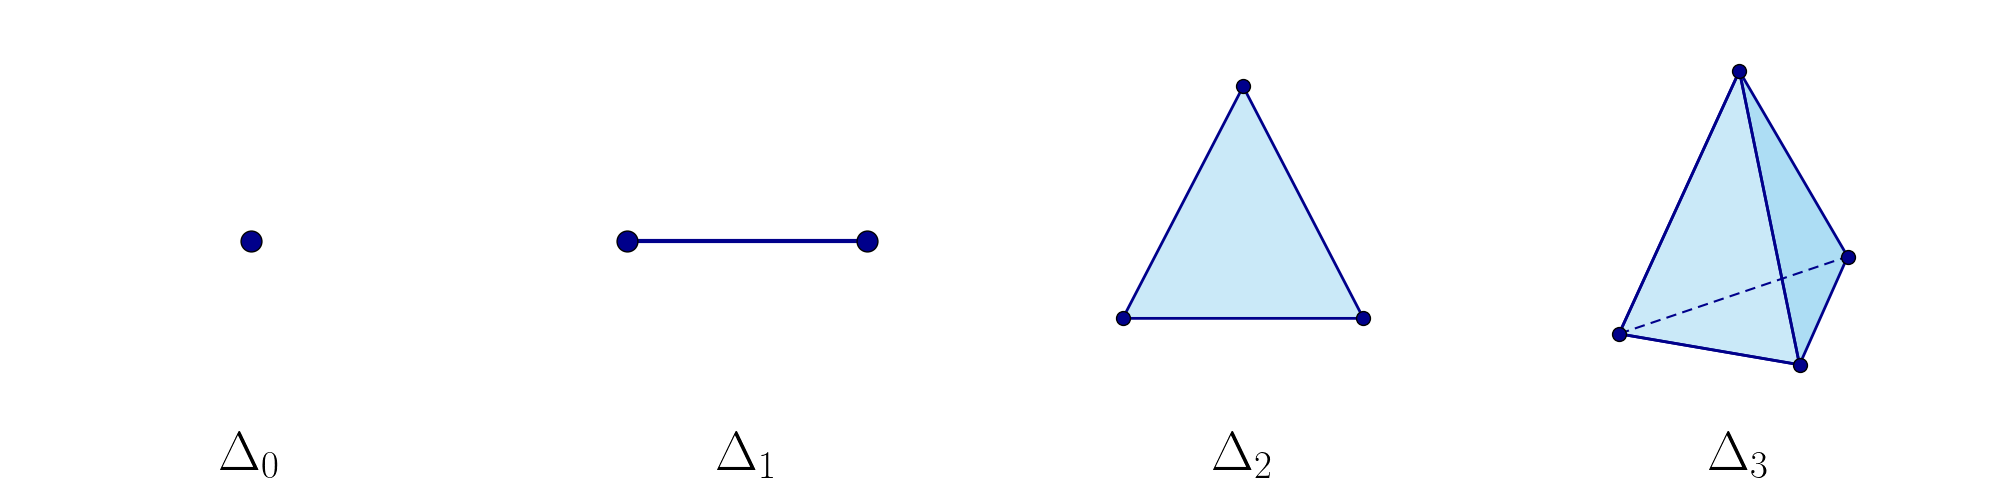
\includegraphics[width=0.8\textwidth]{Imagens/definicao_simplices.png}
  \end{center}
\end{frame}

\begin{frame}{Complexos Simpliciais}
  \textbf{Definição.} Seja $K$ um complexo simplicial com conjunto de vértices $V=\left\{ 1, \dots, n \right\}$. Em $\mathbb{R}^{n+1}$, considere, para cada $i \in \left\{ 0, \cdots, n \right\}$, o vetor $e_i = (0, \dots, 1, 0, \dots, 0)$. Seja $|K|$ o subconjunto de $\mathbb{R}^{n+1}$ definido por:
  \begin{align*}
      |K| = \bigcup_{\sigma \in K} \textup{conv}(\{e_j, j \in \sigma\})
  \end{align*}
  onde $\textup{conv}$ representa o fecho convexo.
  Munido da topologia de subespaço, $(|K|, \tau_{|K|})$ é um espaço topológico, que denominamos realização topológica de $K$.
\end{frame}

\begin{frame}{Complexos Simpliciais}
  \textbf{Definição.} Seja $(X, \mathcal{T})$ um espaço topológico. Uma triangulação de $X$ é um complexo simplicial $K$ tal que sua realização topológica $(|K|, \mathcal{T}_{|K|})$ é homeomorfa a $(X, \mathcal{T})$.
  
  \vspace{0.3cm}

  \begin{figure}
    \centering
    \begin{minipage}{0.48\textwidth}
      \centering
      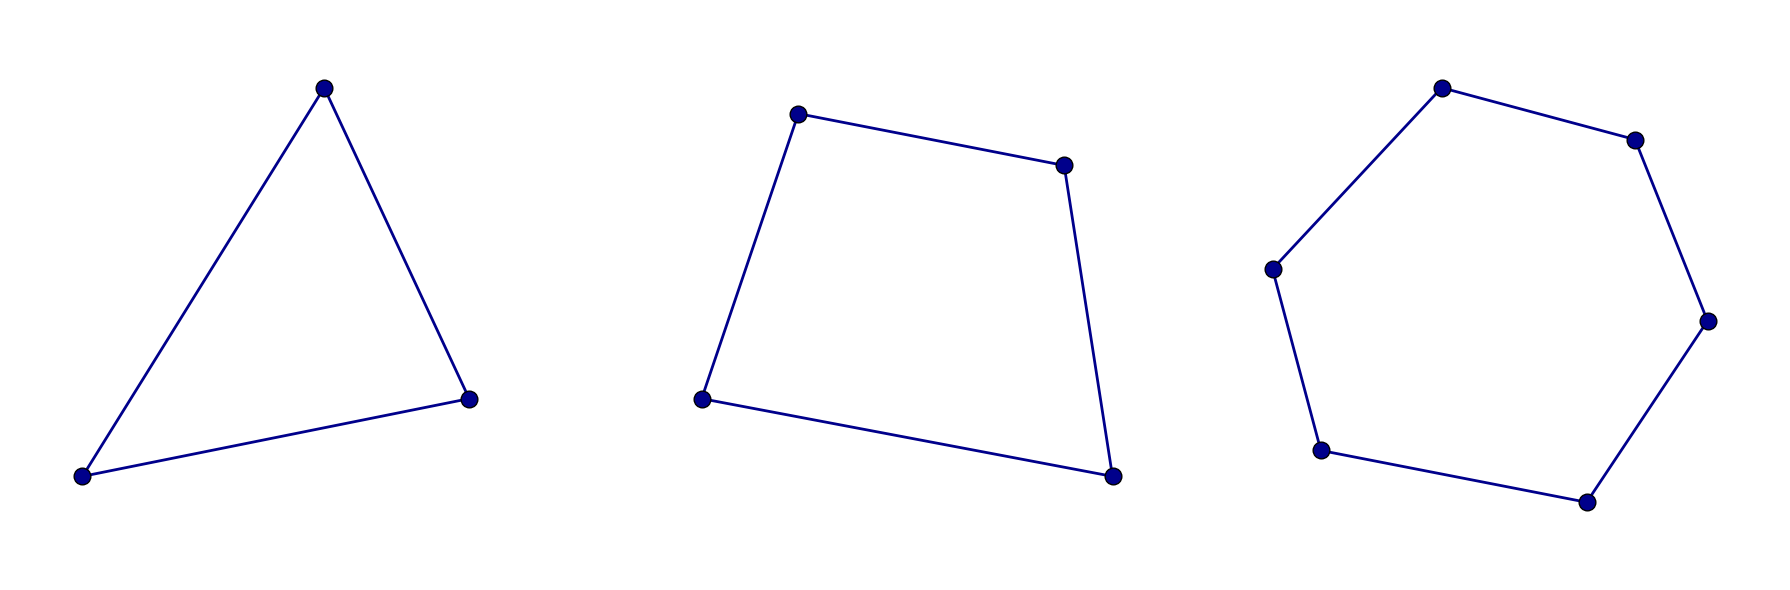
\includegraphics[width=\textwidth]{Imagens/triangulacao_circulo.png}
    \end{minipage}
    \hfill
    \vrule
    \hfill
    \begin{minipage}{0.48\textwidth}
      \centering
      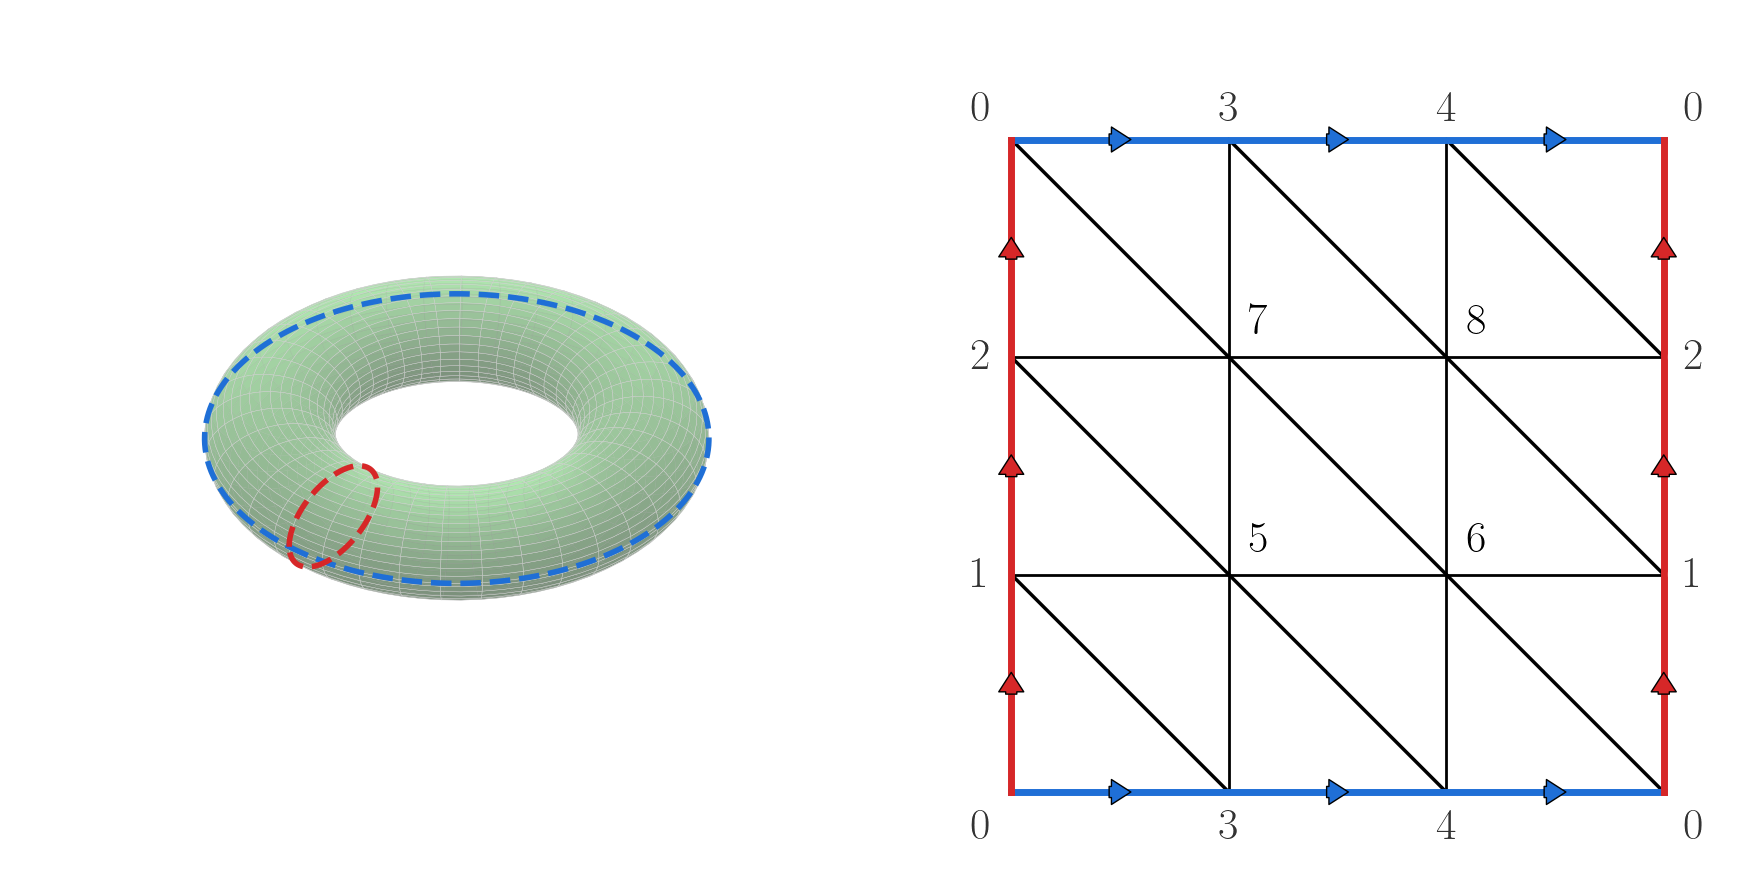
\includegraphics[width=\textwidth]{Imagens/triangulacao_toru.png}
    \end{minipage}
    \caption{À esquerda, a triangulação de um círculo. À direita, a triangulação de um toro.}
  \end{figure}
\end{frame}

\begin{frame}{Cadeias, Fronteira e Homologia}
  \textbf{Definição}. Seja $K$ um complexo simplicial e $n \geq 0$. O conjunto de $n$-cadeias de $K$, denotado $C_n(K)$, é o conjunto cujos elementos são as somas formais:
  \[
  \sum_{\sigma \in K_{(n)}} \epsilon_\sigma \cdot \sigma, \quad \text{onde } \forall \sigma \in K_{(n)},\; \epsilon_\sigma \in \mathbb{Z}/2\mathbb{Z}.
  \]
  
  \textbf{Definição}. Seja $n \geq 1$ e $\sigma = [x_0, \ldots, x_n] \in K_{(n)}$ um símplexo de dimensão $n$. A fronteira de $\sigma$ é o elemento de $C_{n-1}(K)$ definido por:
  \[
  \partial_n \sigma = \sum_{\substack{\tau \subset \sigma \\ |\tau| = |\sigma| - 1}} \tau.
  \]
  O operador $\partial_n$ estende-se por linearidade a uma aplicação linear $\partial_n: C_n(K) \to C_{n-1}(K)$.
\end{frame}

\begin{frame}{Cadeias, Fronteira e Homologia}
  Um exemplo das 1-cadeias $C_1(K)$ do complexo $K = \left\{[0], [1], [2], [0, 1], [0, 2]\right\}$.

  \begin{figure}
    \centering
    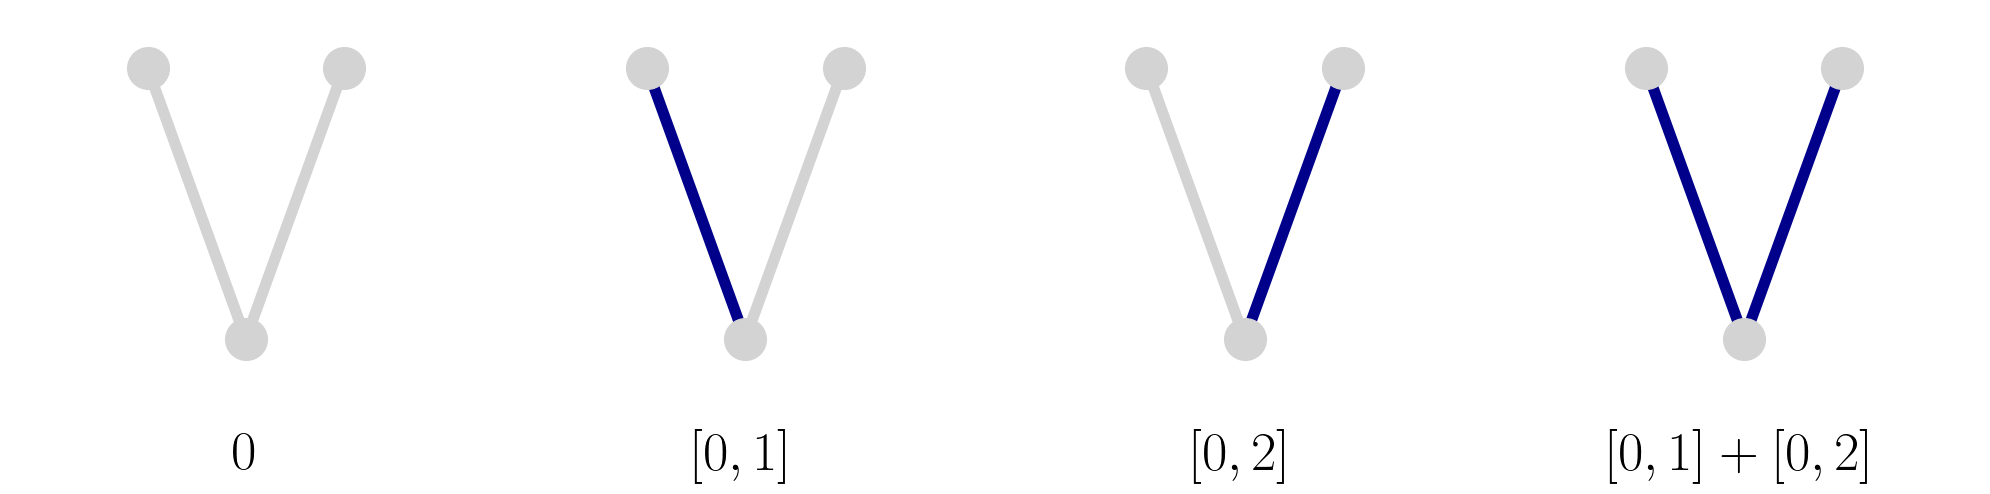
\includegraphics[width=0.6\textwidth]{Imagens/fases_n_cadeias1.png} 
  \end{figure}
  \hfill

  Considerando o complexo $K = \{[0], [1], [2], [3], [0, 1], [0, 2], [1, 2], [1, 3], [2, 3], [0, 1, 2]\}$, aplicando o operador fronteira no simplexo $[0,1]$, temos:
    \begin{figure}
    \centering
    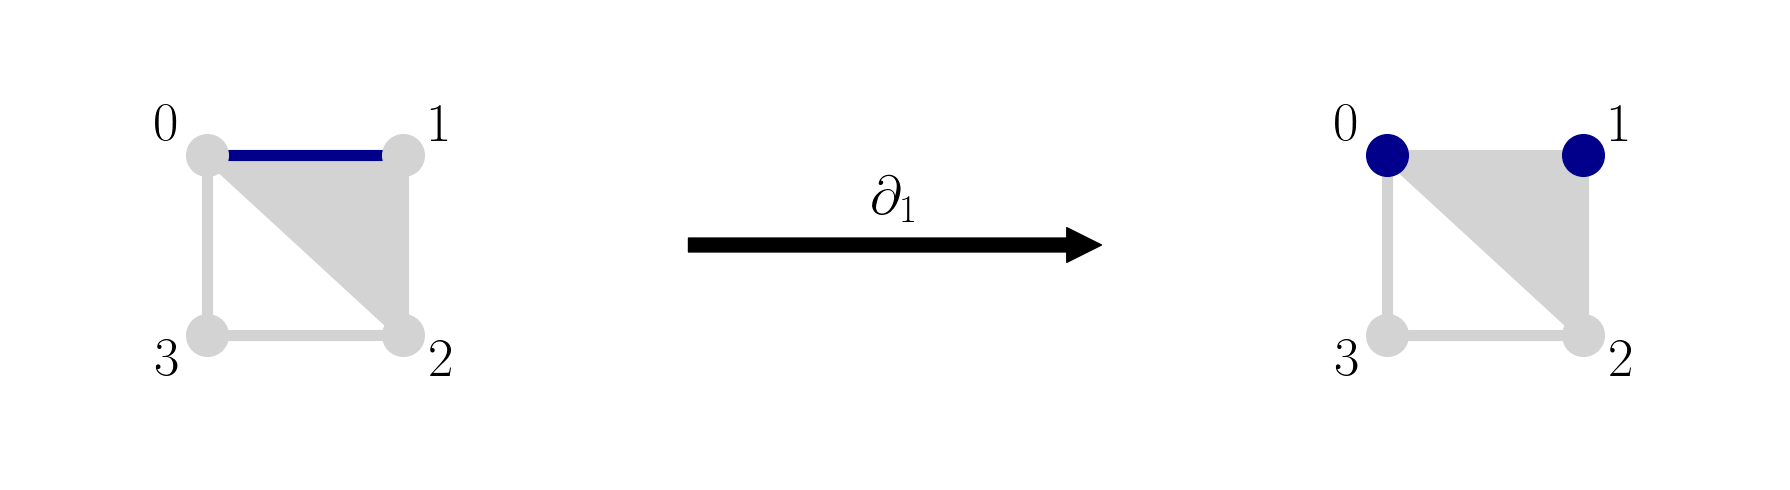
\includegraphics[width=0.6\textwidth]{Imagens/fronteiras_ex1.png}
  \end{figure}
\end{frame}

\begin{frame}{Cadeias, Fronteira e Homologia}
  \textbf{Definição.} Seja $K$ um complexo simplicial. O $n$-ésimo grupo de homologia de $K$ é o quociente:
    \begin{align*}
        H_n(K) = Z_n(K) / B_n(K).
    \end{align*}
    A dimensão deste espaço vetorial é o $n$-ésimo número de Betti, dado por $\beta_n(K) = \dim H_n(K) = \dim Z_n(K) - \dim B_n(K)$. Geometricamente, $\beta_0$ conta o número de componentes conexas, $\beta_1$ o número de ``buracos'' ou ciclos unidimensionais, e $\beta_2$ o número de cavidades fechadas.

    \begin{figure}
      \centering
      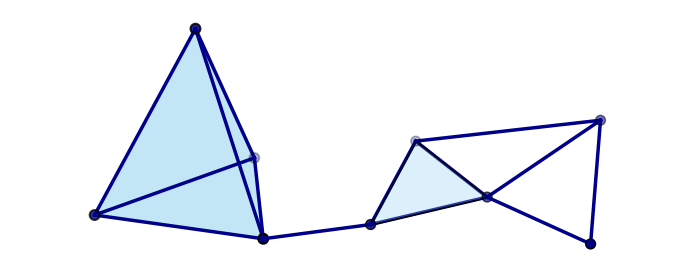
\includegraphics[width=0.6\textwidth]{Imagens/exemplo_n_betti.png}
    \end{figure}
\end{frame}

\begin{frame}{Inferência Topológica: do Ponto à Forma}
  \textbf{Definição.} Seja $X \subset \mathbb{R}^n$ e $t \geq 0$. O $t$-espessamento de $X$, denotado $X^t$, é o conjunto de pontos do espaço ambiente com o máximo de distância $t$ de $X$:
    \[
    X^t = \{y \in \mathbb{R}^n \mid \exists x \in X,\, \|x - y\| \leq t\} = \bigcup_{x \in X} \overline{\mathcal{B}}(x, t).
    \]
    Lê-se que $X^t$ é uma união de bolas fechadas centradas em cada ponto de $X$.
  
  \begin{figure}
    \centering
      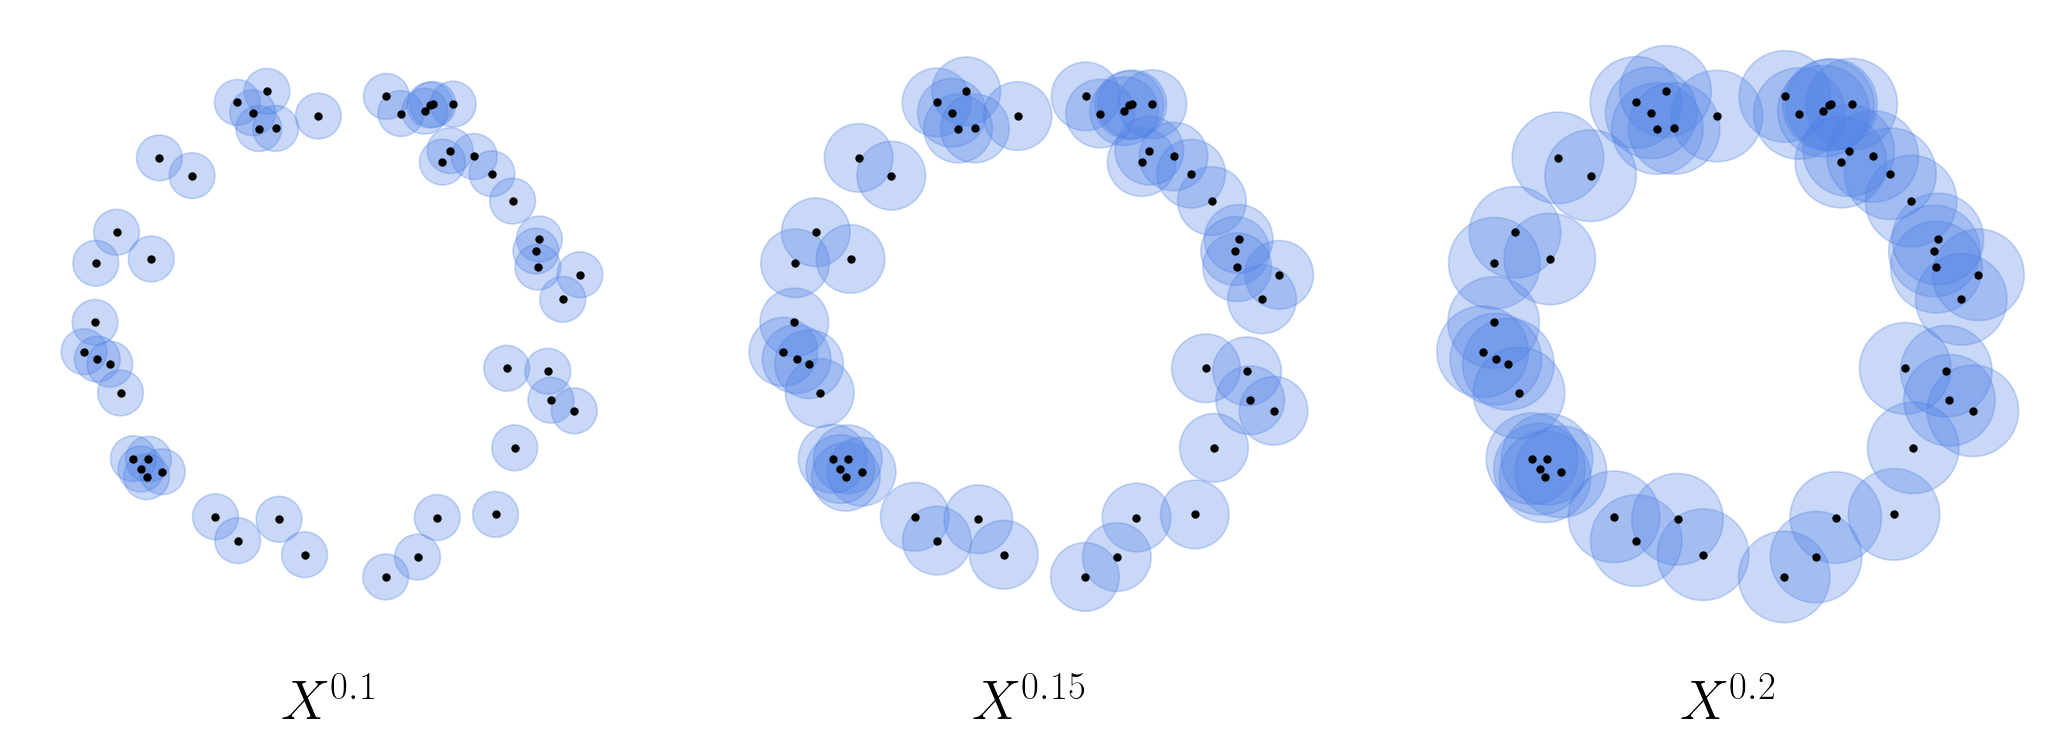
\includegraphics[width=0.7\textwidth]{Imagens/epessamentos_x.png}
  \end{figure}
\end{frame}

\begin{frame}{Inferência Topológica: do Ponto à Forma}
  \textbf{Teorema do Nervo.} Suponha que $X$ seja um subconjunto de $\mathbb{R}^n$. Considere uma cobertura $\mathcal{U} = \left\{U_i\right\}_{1\leq i \leq N}$ de $X$ tal que cada um dos $U_i$ são bolas fechadas e convexas. Então $\mathcal{N}(\mathcal{U})$ é homotopia equivalente a $X$.
  \begin{figure}
    \centering
      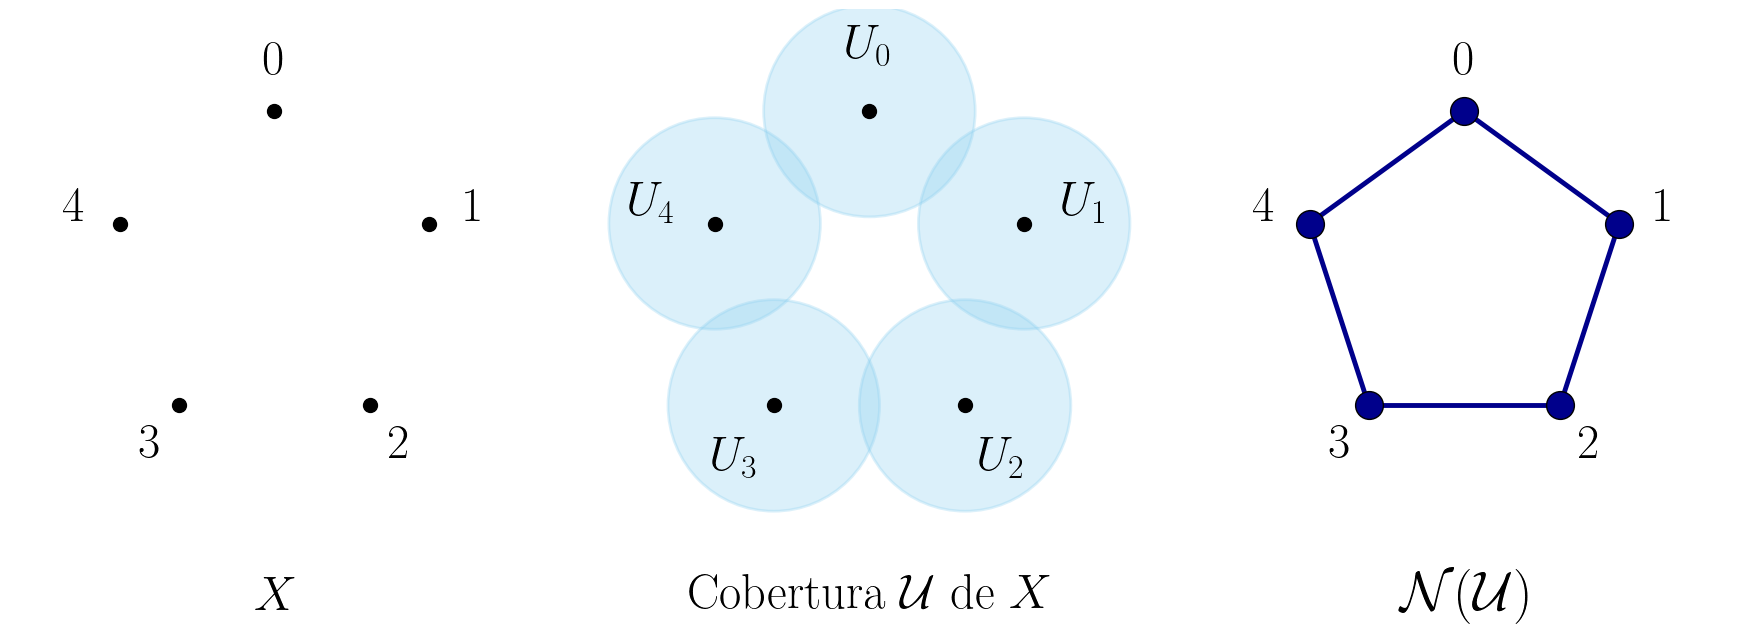
\includegraphics[width=0.7\textwidth]{Imagens/cobertura_nervo.png}
  \end{figure}

  Isso permite recuperar $H_i(X)$ a partir de $H_i(X^t)$, para $t$ adequado.
\end{frame}

\begin{frame}{Complexo de Čech e de Rips}
  \textbf{Definição. (Complexo de Čech).}Sejam $X \subset \mathbb{R}^n$ finito e $t \geq 0$. Considere a coleção $\mathcal{V}^t = \{\overline{\mathcal{B}}(x,t) \mid x \in X\}$. O nervo desta coleção é denotado $\check{\mathrm{C}}\mathrm{ech}^t(X)$ e é chamado de complexo de \v{C}ech de $X$ no instante $t$.

  \vspace{0.3cm}

  \textbf{Definição. (Complexo de Rips).} Sejam $X = \{x_1, \ldots, x_N\} \subset \mathbb{R}^n$ um conjunto finito e $t \geq 0$. O complexo de Rips de $X$ no instante $t$, denotado $\mathrm{Rips}^t(X)$, é o complexo do grafo $G^t = \left(\check{\mathrm{C}}\mathrm{ech}^t(X)\right)$ cujo conjunto de vértices é $\{1, \ldots, N\}$ e cujas arestas são os pares $(i,j)$ tais que a distância entre eles obedece a $\|x_i - x_j\| \leq 2t$.

  \begin{figure}
    \centering
      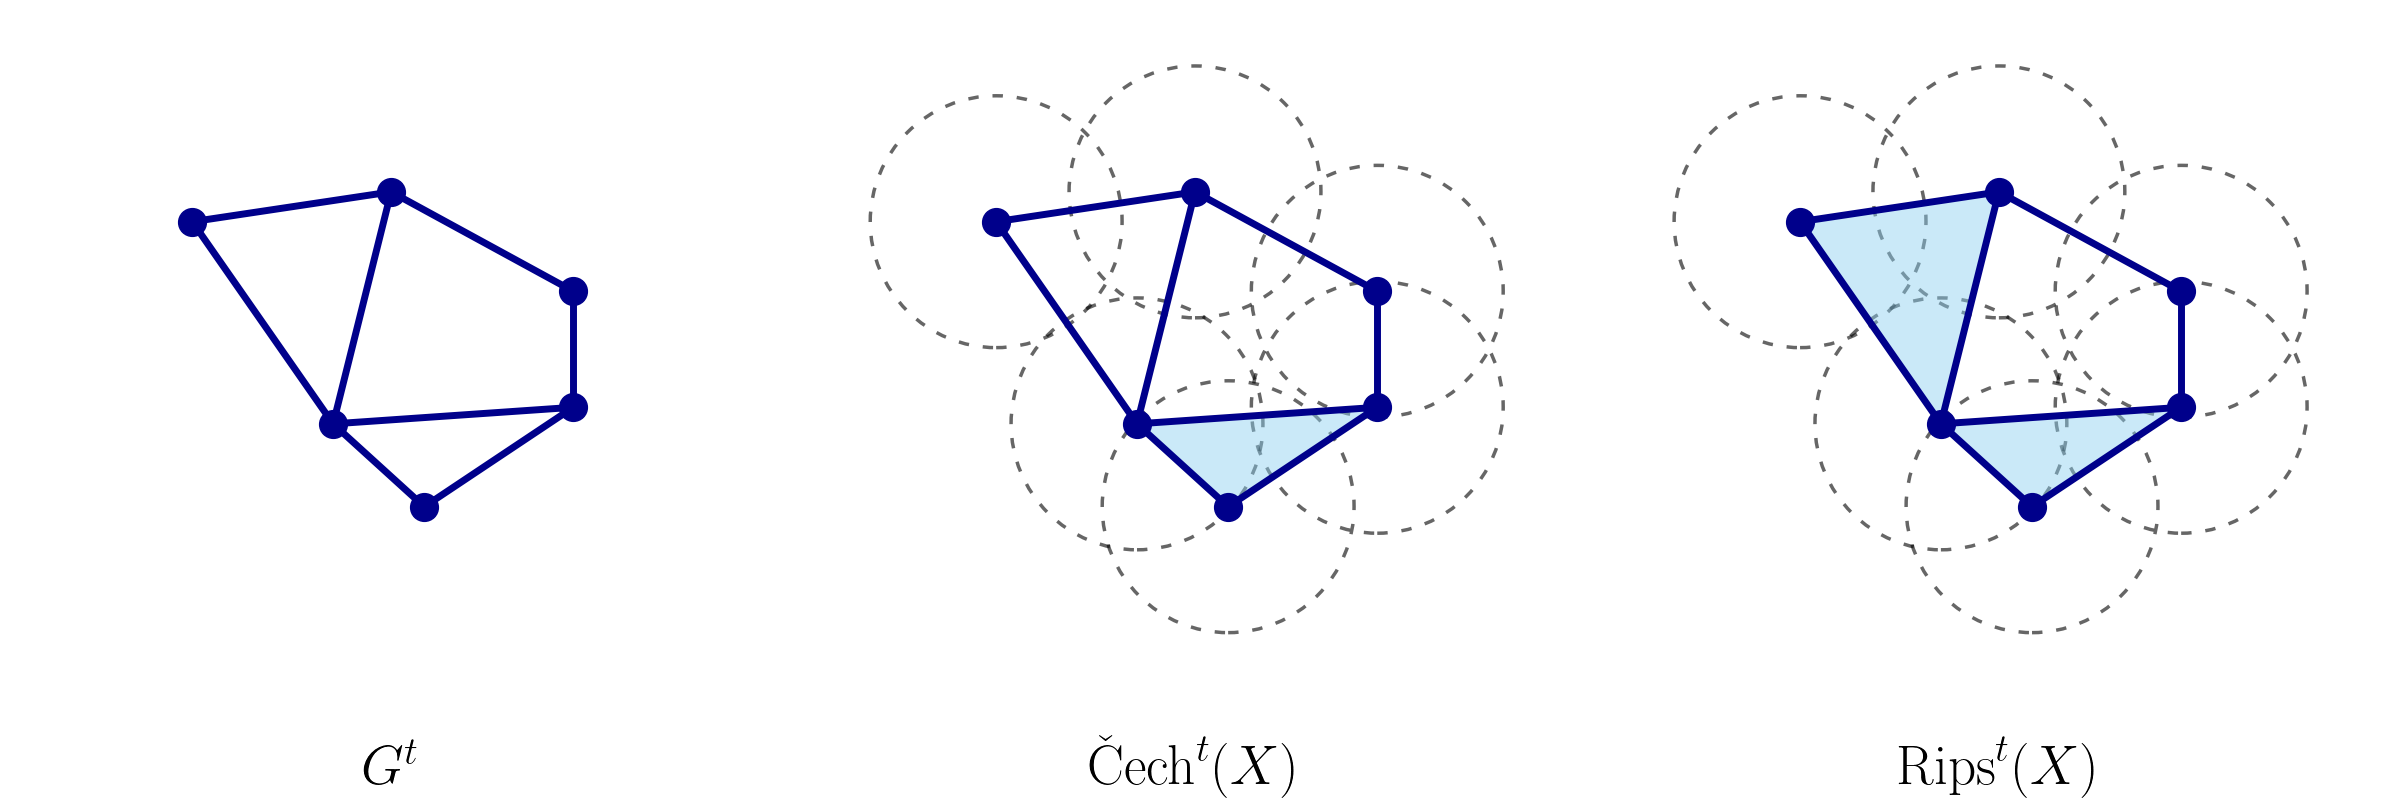
\includegraphics[width=0.7\textwidth]{Imagens/cech_vs_rips.png}
  \end{figure}
\end{frame}


% =====================================================================
\section{Homologia Persistente}
% =====================================================================
\begin{frame}{Curvas de Betti}
  \begin{columns}[T] % [T] alinha as colunas pelo topo
    
    % --- COLUNA DA ESQUERDA (Texto + 2 imagens antigas lado a lado) ---
    \begin{column}{0.5\textwidth}
      \textbf{Definição.} Seja $X \subset \mathbb{R}^n$ e $i\geq 0$. A $i$-ésima curva de Betti de $X$ é a aplicação
      \begin{align*}
          \beta_i(t): \mathbb{R}^+& \longrightarrow \mathbb{N}\\
          &t \longmapsto \beta_i\left(X^t\right)
      \end{align*} 
      Podemos observar essa definição por uma amostra ruidosa de um círculo $X$.
      
      \vspace{0.3cm}
      
      \begin{figure}
        \centering
        \begin{minipage}{0.4\textwidth}
            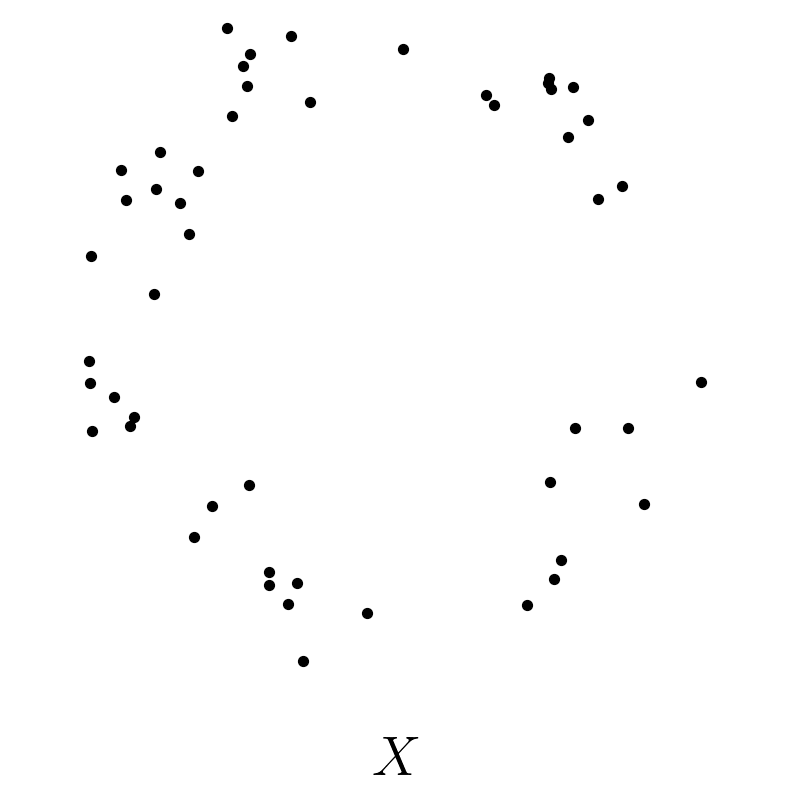
\includegraphics[width=\textwidth]{Imagens/exemplo_curva_betti.png}
        \end{minipage}
        \hfill
        \begin{minipage}{0.4\textwidth}
            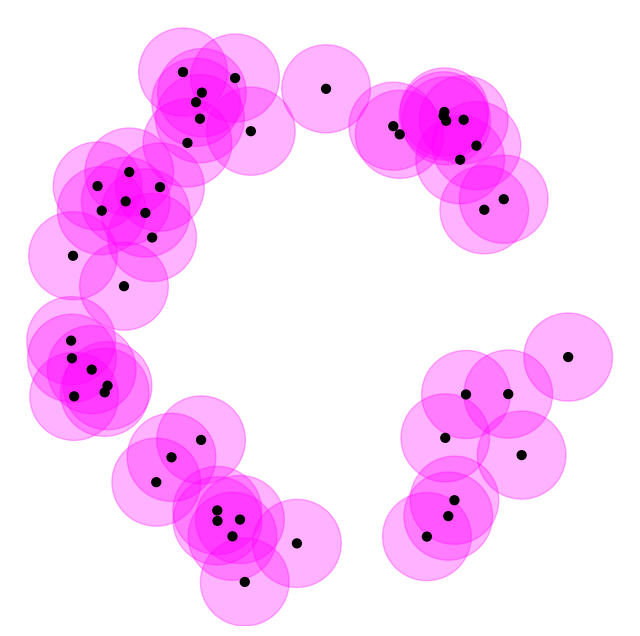
\includegraphics[width=\textwidth]{Imagens/espessamento_betti.png}
        \end{minipage}
      \end{figure}
    \end{column}
    \vrule
    % --- COLUNA DA DIREITA (Novas imagens Betti 0 e Betti 1 EMPILHADAS) ---
    \begin{column}{0.45\textwidth}
      \begin{figure}
        \centering
        
        % Imagem de cima (Betti 0)
        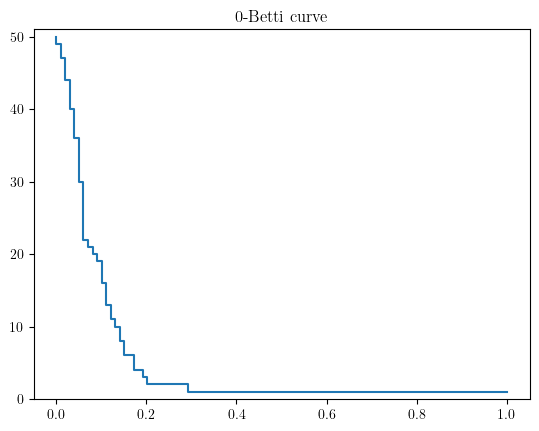
\includegraphics[width=0.6\textwidth]{Imagens/betti0_exemplo.png}
        
        \vspace{0.5cm} % Espaço entre as duas imagens empilhadas
        
        % Imagem de baixo (Betti 1)
        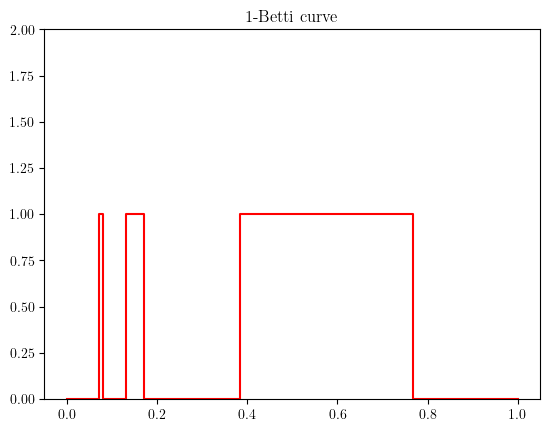
\includegraphics[width=0.6\textwidth]{Imagens/betti1_exemplo.png}
        
      \end{figure}
    \end{column}
    
  \end{columns}
\end{frame}

\begin{frame}{Filtração e Funtorialidade}
    \textbf{Definição.} Uma \textbf{filtração} de um complexo simplicial $E$ é uma família de subcomplexos $\mathbb{X} = (X^t)_{t \in \mathbb{R}^+}$ de $E$ tais que $X_s \subseteq X_t$ sempre que $s \leq t$.
    \vspace{0.3cm}
    
    Aplica-se isso à família de complexos de Vietoris-Rips:
    \[
        X_{t_1} \subseteq X_{t_2} \subseteq X_{t_3} \subseteq \dots \subseteq X_{t_n}
    \]
    
    A inclusão $i: X_s \hookrightarrow X_t$ induz um homomorfismo nos grupos de homologia:
    \[
        (i_*)_k: H_k(X_s) \longrightarrow H_k(X_t)
    \]
    \textbf{Propriedade Funtorial:} Permite rastrear a evolução dos ciclos $H_k$, identificando o momento exato em que um ciclo nasce e morre.
\end{frame}

\begin{frame}{Módulos de Persistência e Barcodes}
    \textbf{Definição. (Módulo de Persistência)} A coleção dos espaços vetoriais $V_t = H_k(X_t)$ acompanhada das aplicações induzidas $v_{s,t}: V_s \to V_t$.
    \vspace{0.5cm}

    \textbf{Teorema da Decomposição} Todo módulo de persistência de dimensão finita decompoe-se de forma única em somas diretas de módulos intervalares $\mathbb{I}(b_i, d_i)$:
    \[
        V \cong \bigoplus_{i=1}^m \mathbb{I}(b_i, d_i)
    \]
    \textbf{Representações Equivalentes:}
    \begin{itemize}
        \item \textbf{Código de Barras (Barcode):} Conjunto de intervalos de vida $[b_i, d_i)$.
        \item \textbf{Diagrama de Persistência:} Multiconjunto de pontos $(b_i, d_i) \in \mathbb{R}^2$.
    \end{itemize}
    \vspace{0.2cm}
\end{frame}

\begin{frame}{Módulos de Persistência e Barcodes}
  À medida que o parâmetro de filtração $t$ avança, a topologia do complexo se altera com o surgimento e desaparecimento de ciclos homológicos. Esse histórico é sintetizado nos resumos de persistência:

    \vspace{0.2cm}

    \begin{figure}[H]
        \centering
        % --- PRIMEIRA LINHA: Progressão da Filtração (4 imagens) ---
        \begin{minipage}[b]{0.23\textwidth}
            \centering
            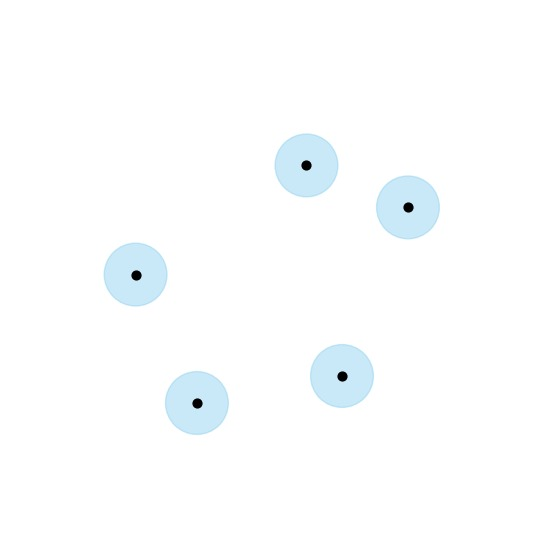
\includegraphics[width=\textwidth]{Imagens/barcode_simplexo_0.5.png}
            \caption{\scriptsize $t = 0.50$}
        \end{minipage}\hfill
        \begin{minipage}[b]{0.23\textwidth}
            \centering
            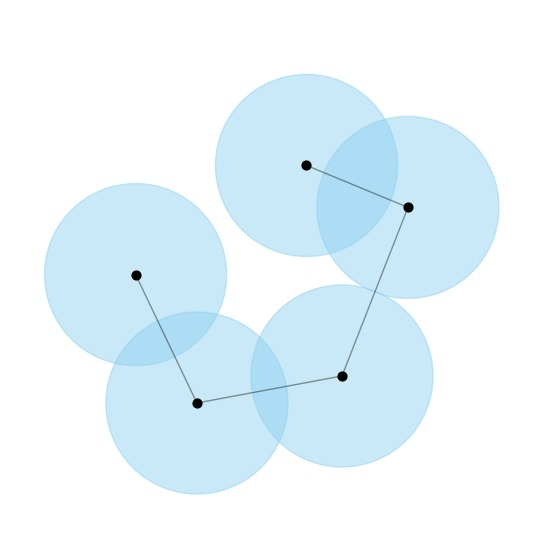
\includegraphics[width=\textwidth]{Imagens/barcode_simplexo_1.45.png}
            \caption{\scriptsize $t = 1.45$}
        \end{minipage}\hfill
        \begin{minipage}[b]{0.23\textwidth}
            \centering
            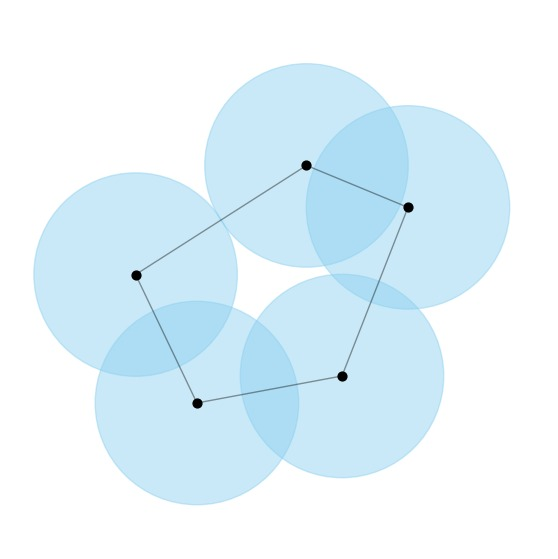
\includegraphics[width=\textwidth]{Imagens/barcode_simplexo_1.62.png}
            \caption{\scriptsize $t = 1.62$}
        \end{minipage}\hfill
        \begin{minipage}[b]{0.23\textwidth}
            \centering
            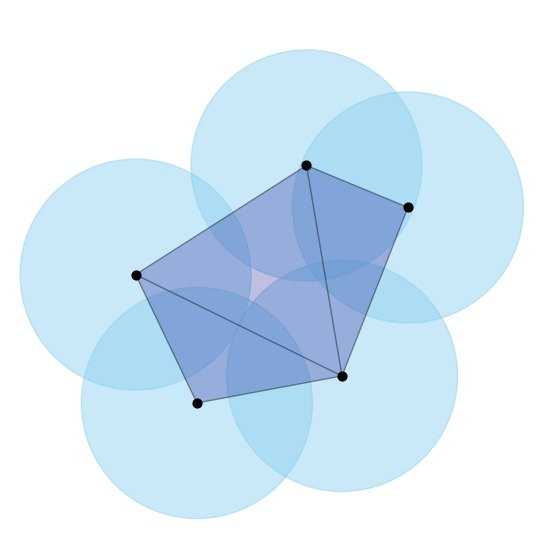
\includegraphics[width=\textwidth]{Imagens/barcode_simplexo_1.84.png}
            \caption{\scriptsize $t = 1.84$}
        \end{minipage}

        \vspace{0.3cm}
      \end{figure}
\end{frame}

\begin{frame}{Módulos de Persistência e Barcodes}
  \begin{figure}
    \centering
    % --- SEGUNDA LINHA: Barcode e Diagrama de Persistência (2 imagens) ---
        \begin{minipage}[b]{0.45\textwidth}
            \centering
            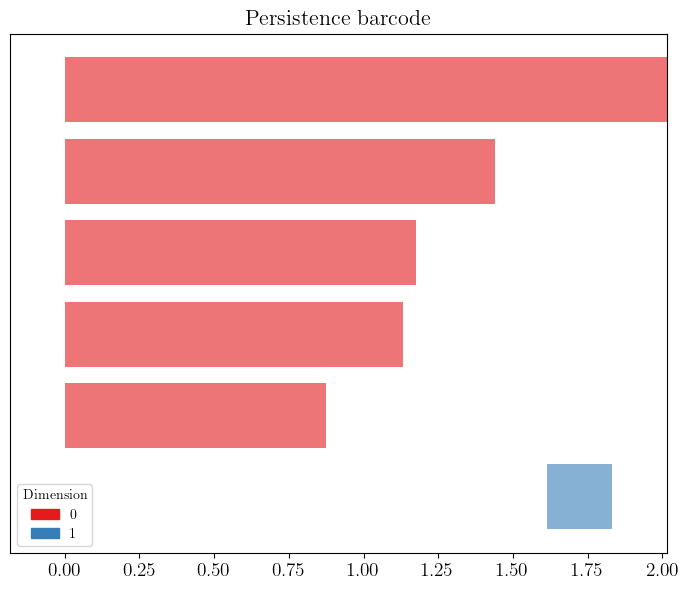
\includegraphics[width=\textwidth]{Imagens/barocode_def.png}
            \caption{Código de Barras (\emph{Barcode})}
        \end{minipage}\hfill
        \begin{minipage}[b]{0.45\textwidth}
            \centering
            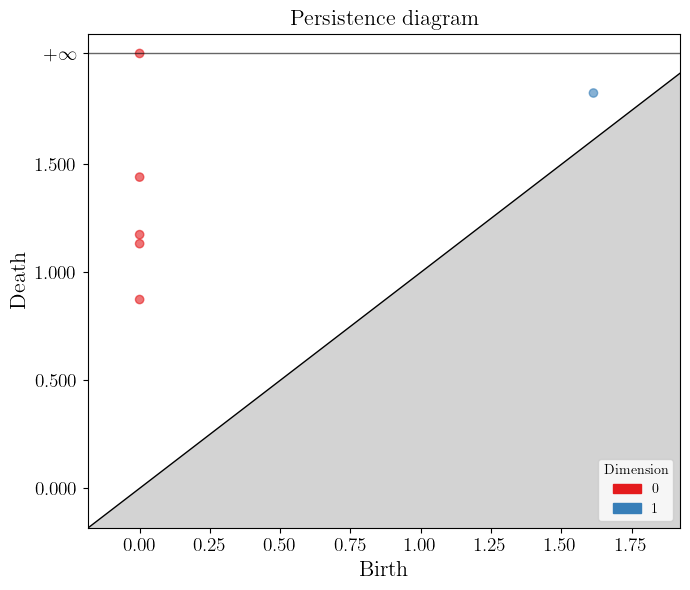
\includegraphics[width=\textwidth]{Imagens/diagrama_def.png}
            \caption{Diagrama de Persistência}
        \end{minipage}
  \end{figure}
\end{frame}

\begin{frame}{Paisagens de Persistência (Persistence Landscapes)}
  \textbf{Definição.} Dado um diagrama de persistência com intervalos $\mathcal{B} = \{(b_i, d_i)\}_{i=1}^m$, define-se para cada ponto a função auxiliar:
    \[
        f_{(b,d)}(t) = \max(0, \min(t-b,\; d-t)).
    \]
    A paisagem de persistência é a sequência de funções $\lambda_k : \mathbb{R} \to \mathbb{R}$ definidas por:
    \[
        \lambda_k(t) = k\text{-ésimo maior valor do conjunto } \{f_{(b_i,d_i)}(t)\}_{i=1}^m,
    \]
    adotando $\lambda_k(t) = 0$ caso $k > m$.

    \begin{figure}[H]
        \centering
        \begin{minipage}[b]{0.4\textwidth}
            \centering
            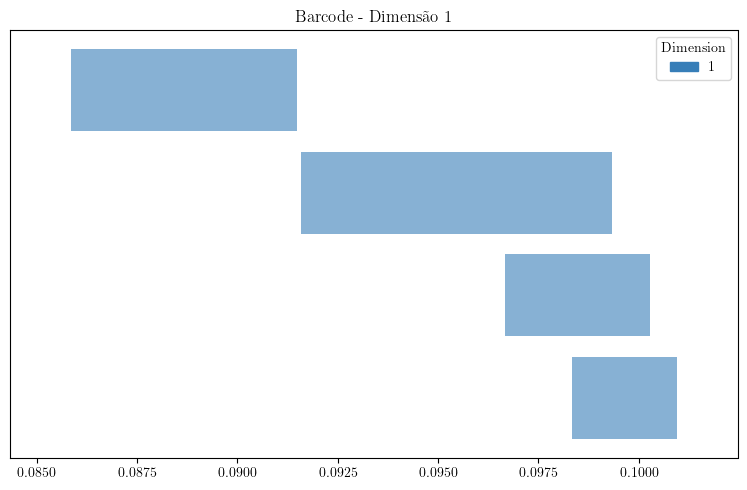
\includegraphics[width=\linewidth]{Imagens/barcode_landscape.png}
        \end{minipage}\hfill
        \begin{minipage}[b]{0.4\textwidth}
            \centering
            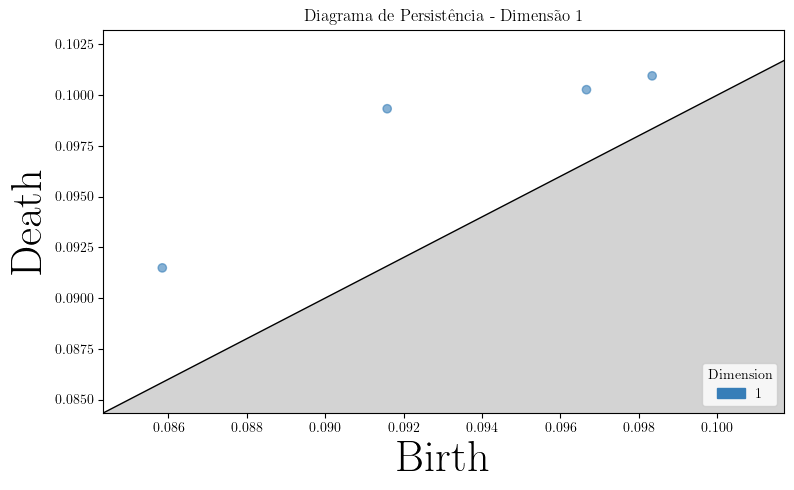
\includegraphics[width=\linewidth]{Imagens/diagrama_landscape.png}
        \end{minipage}
    \end{figure}
\end{frame}

\begin{frame}{Paisagens de Persistência (Persistence Landscapes)}
  \vfill
    \begin{figure}[H]
        \centering
        % --- COLUNA DA ESQUERDA (2 imagens empilhadas) ---
        \begin{minipage}[c]{0.38\textwidth}
            \centering
            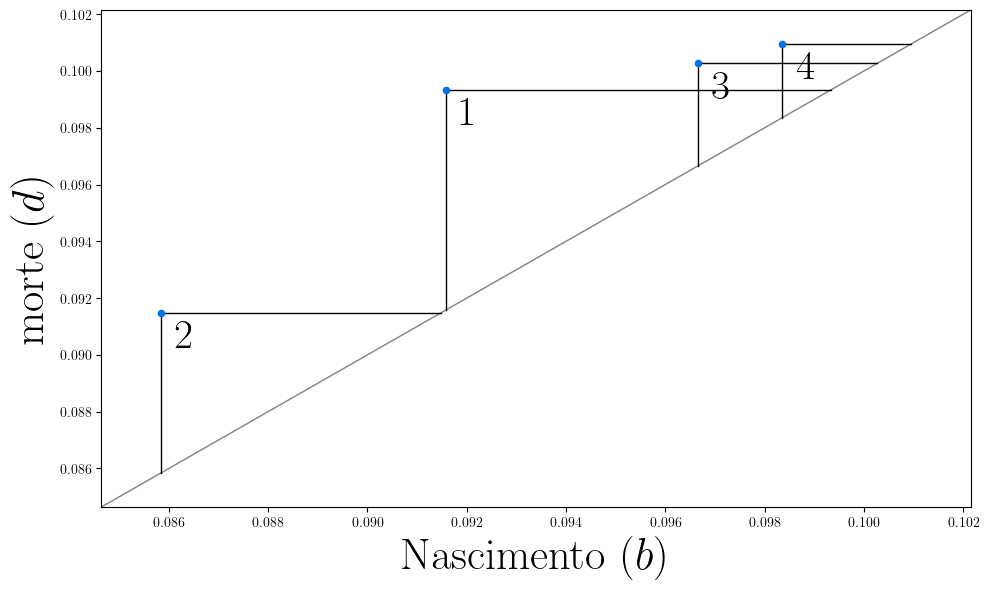
\includegraphics[width=\linewidth]{Imagens/triangulacao_diagrama.png}
            
            \vspace{0.3cm} % Espaçamento vertical entre as duas imagens da esquerda
            
            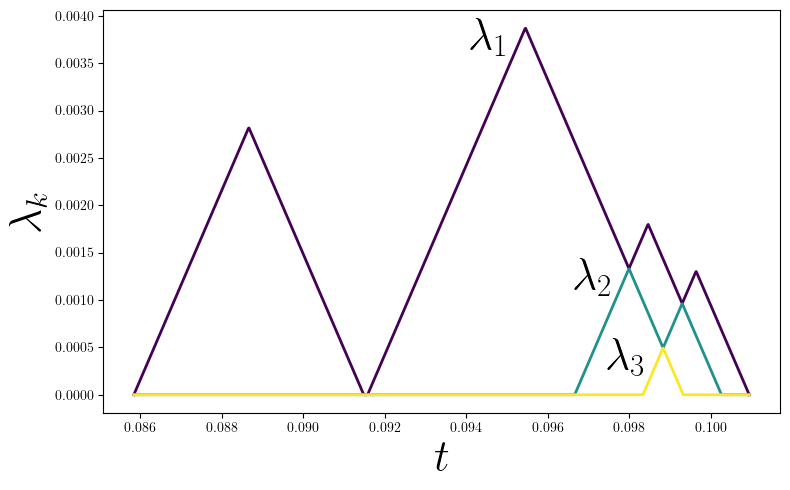
\includegraphics[width=\linewidth]{Imagens/landscapes_2d.png}
        \end{minipage}\hfill
        % --- COLUNA DA DIREITA (1 imagem) ---
        \begin{minipage}[c]{0.50\textwidth}
            \centering
            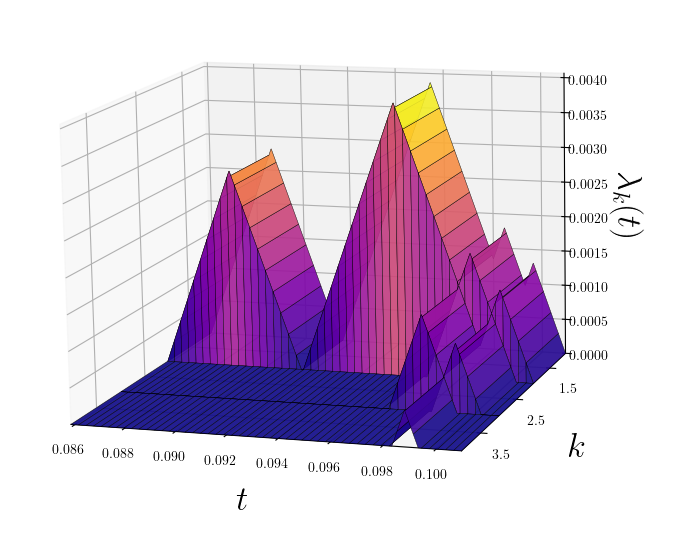
\includegraphics[width=\linewidth]{Imagens/landscapes_3d.png}
        \end{minipage}
    \end{figure}
    \vfill
\end{frame}

\begin{frame}{Paisagens de Persistência (Persistence Landscapes)}
    Essa vetorização através das Paisagens de Persitência nos dá as seguintes vantagens:
    \begin{itemize}
        \item Mapeia a topologia não-linear em um espaço de Banach $L^p(\mathbb{N} \times \mathbb{R})$;
        \item Para $p=2$: Espaço de \textbf{Hilbert} $\Rightarrow$ produto interno $\langle \lambda, \lambda'\rangle_{L^2}$ bem definido;
        \item Permite o uso direto de Máquinas de Vetores de Suporte (SVM) e Análise de Componentes Principais (PCA).
    \end{itemize}
\end{frame}

% =====================================================================
\section{Inferência Estatística}
% =====================================================================

\begin{frame}{Variável Aleatória Topológica e Hipóteses}
  Área total sob a paisagem de persistência:
  \[
    X = \sum_{k=1}^{\infty} \int_{\mathbb R} \lambda_k(t)\, dt
  \]
  \textbf{Teste de hipóteses} entre as populações Fechada ($\mu_1$) e Aberta ($\mu_2$):
  \[
    H_0: \mu_1 = \mu_2 \qquad \text{vs.} \qquad H_a: \mu_1 \neq \mu_2
  \]
  Amostra pequena ($n=14$) $\Rightarrow$ normalidade não garantida $\Rightarrow$ \textbf{teste não-paramétrico}.
\end{frame}

\begin{frame}{Teste de Permutação}
  \[
    T_{\mathrm{obs}} = |\bar X_1 - \bar X_2|, \qquad
    \text{Valor-p} = \frac{1}{M}\sum_{i=1}^{M} \mathbb{I}(T_i \geq T_{\mathrm{obs}})
  \]
  \begin{itemize}
    \item $n=14$ ($7$ Apo $+ 7$ Holo) $\Rightarrow \binom{14}{7} = 3432$ permutações possíveis;
    \item Não assume distribuição prévia dos dados;
    \item Rejeição de $H_0$ (valor-p pequeno) $\Rightarrow$ evidência estatística de separabilidade das assinaturas topológicas.
  \end{itemize}
\end{frame}

% =====================================================================
\section{Redução de Dimensionalidade e Aprendizado de Máquina}
% =====================================================================

\begin{frame}{ISOMAP e Dimensionalidade Intrínseca}
  \begin{itemize}
    \item PCA/MDS clássico assumem geometria euclidiana $\to$ distorcem a variedade da proteína.
    \item \textbf{ISOMAP}: grafo de vizinhança $\to$ distâncias geodésicas (Dijkstra/Floyd-Warshall) $\to$ MDS clássico.
    \item Gráfico Scree indica a dimensão intrínseca ótima (ponto de ``cotovelo'').
    \item Usado apenas para diagnóstico visual (não admite projeção \textit{out-of-sample}).
  \end{itemize}
  \begin{figure}
    \centering
    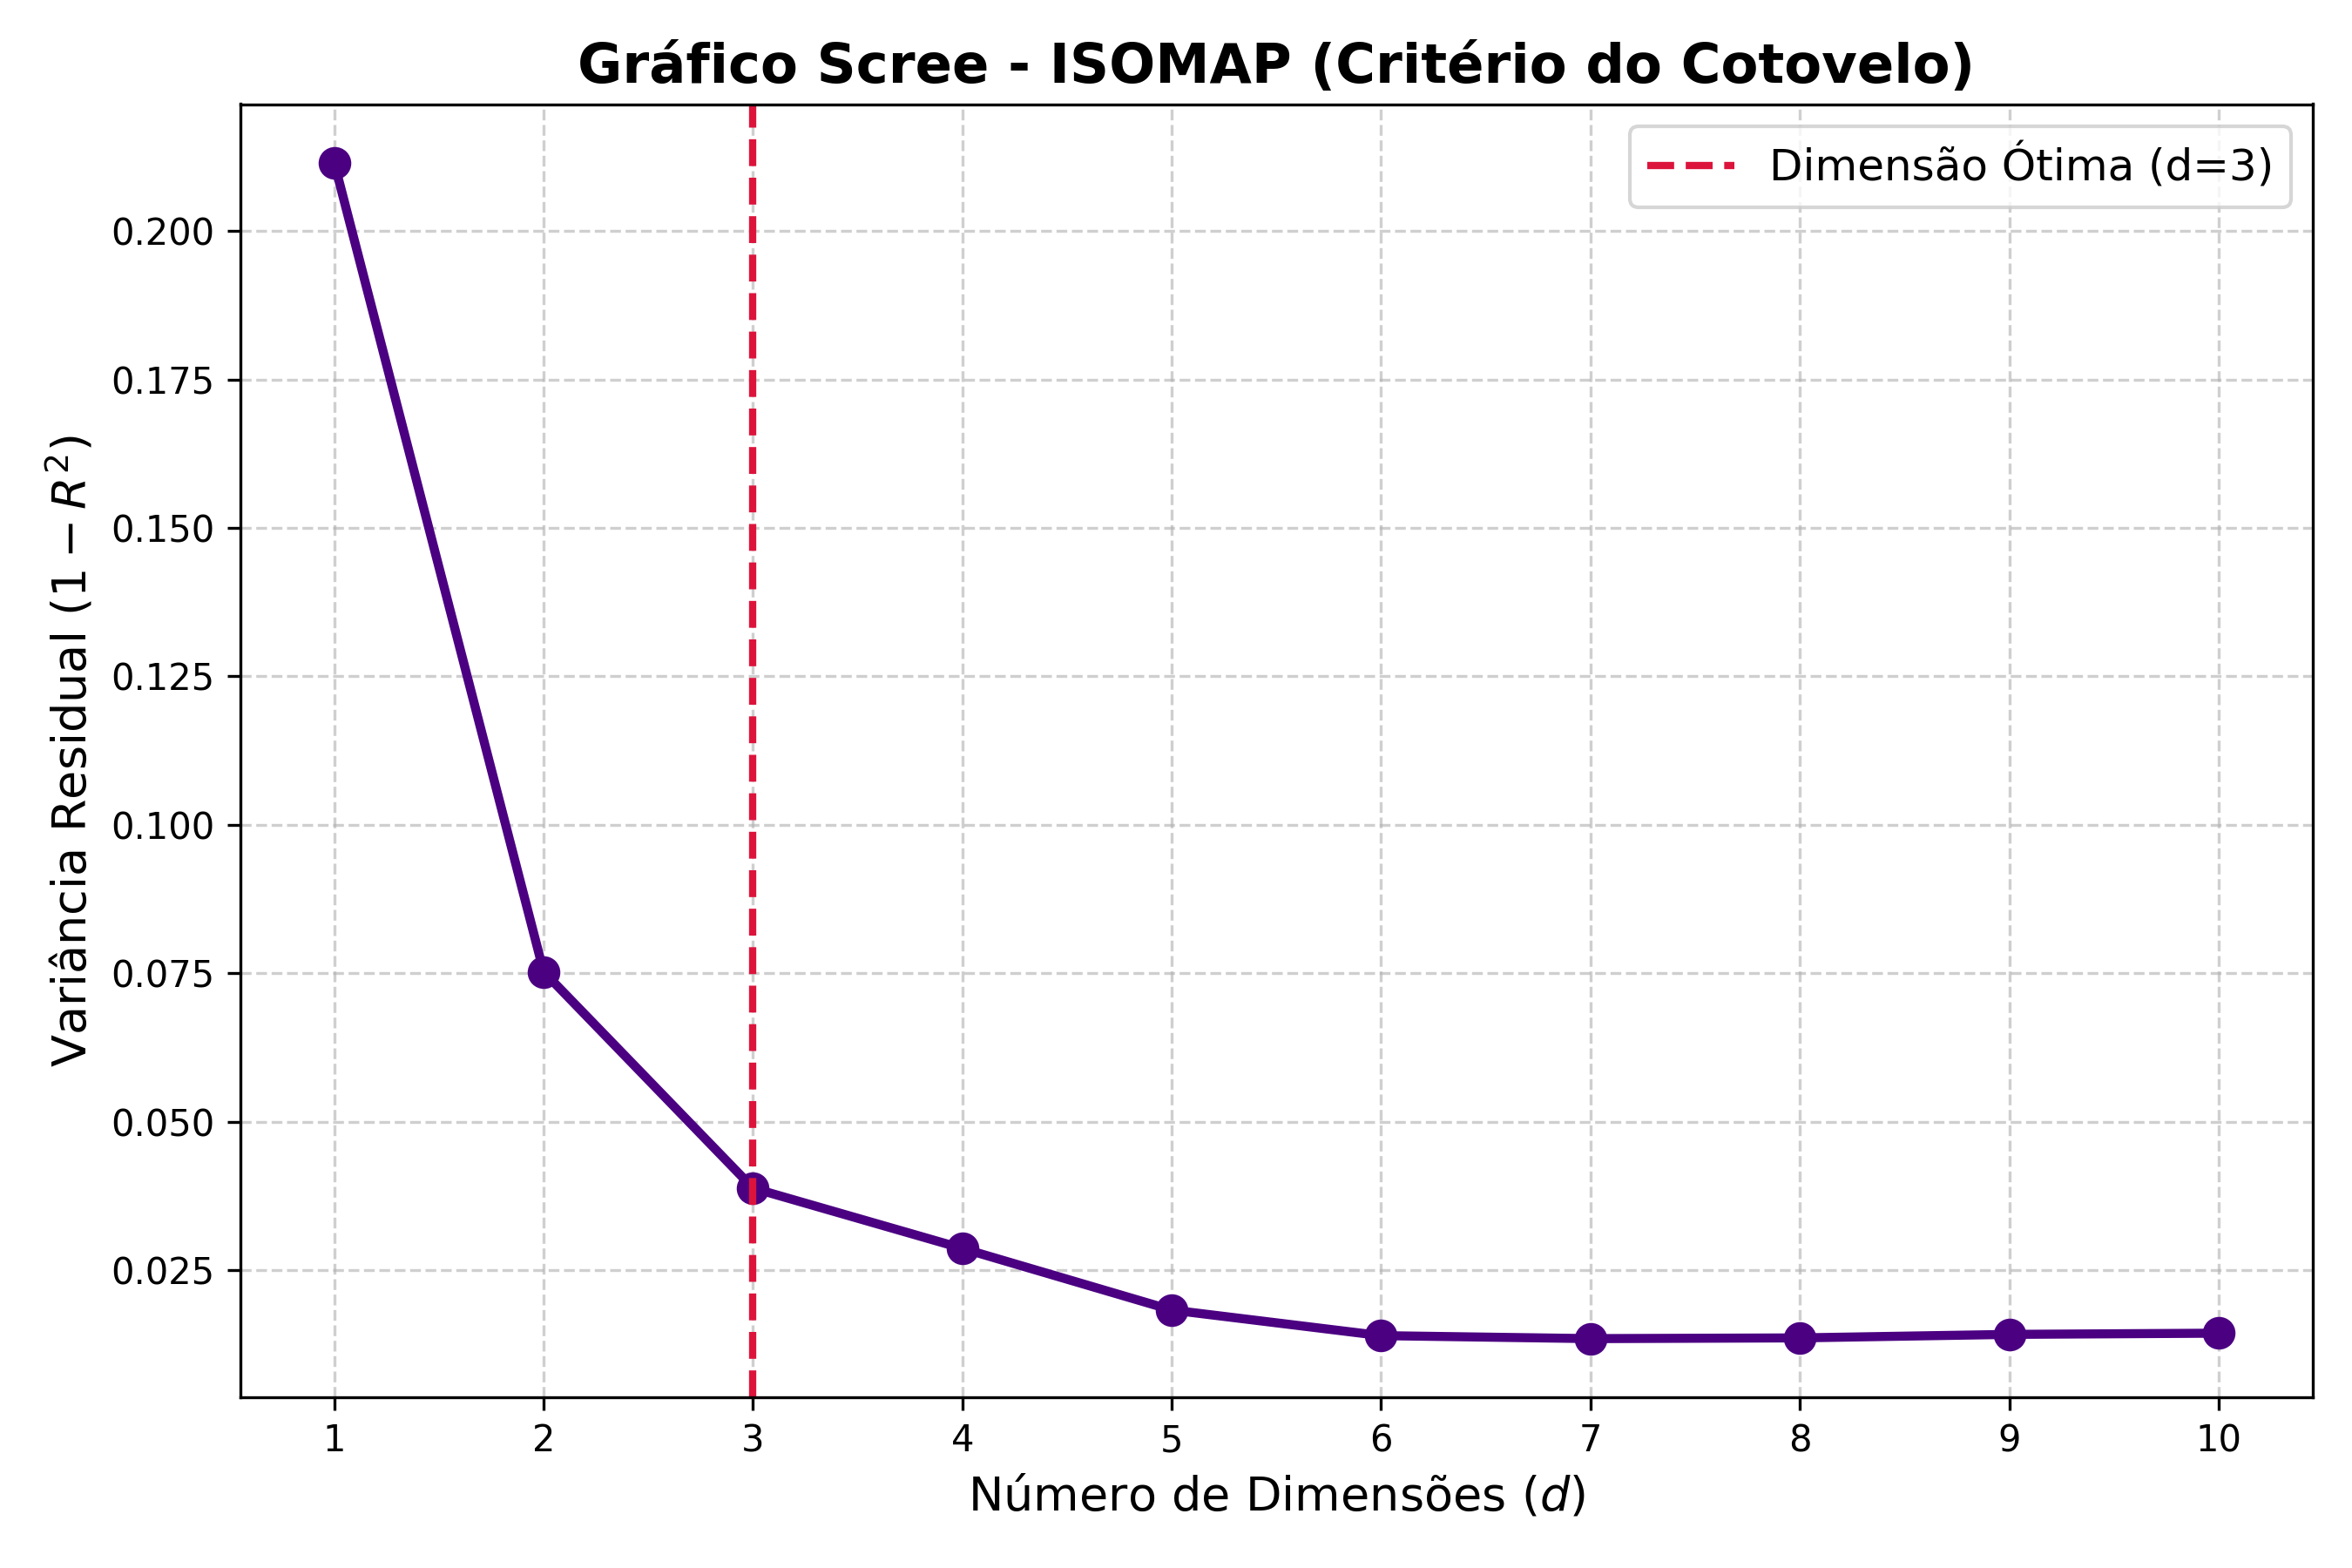
\includegraphics[width=0.43\textwidth]{Imagens/grafico_scree_isomap.png}
  \end{figure}
\end{frame}

\begin{frame}{SVM: Margem Rígida}
    \vfill
    \begin{minipage}[c]{0.52\textwidth}
        Hiperplano separador: 
        \[ f(x) = w\cdot x + b = 0 \]
        com $y_i(w\cdot x_i + b)\geq 1$.

        \[
            \min_{w,b}\ \tfrac{1}{2}\|w\|^2 \quad \text{s.t.} \quad y_i(w\cdot x_i+b)\geq 1,\ \forall i
        \]

        \begin{itemize}
            \item \textbf{Margem geométrica:} $\dfrac{2}{\|w\|}$;
            \item \textbf{Problema dual:} resolvido via multiplicadores de Lagrange $\alpha_i$;
            \item \textbf{Vetores de suporte:} pontos com $\alpha_i^* > 0$.
        \end{itemize}
    \end{minipage}\hfill
    \begin{minipage}[c]{0.45\textwidth}
        \centering
        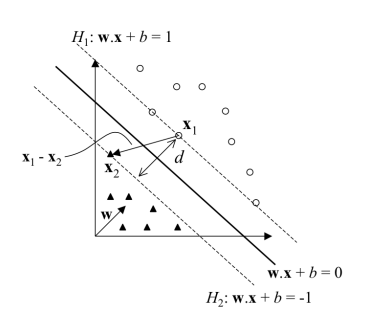
\includegraphics[width=\linewidth]{Imagens/hiperplano_h1_h2.png}
    \end{minipage}
    \vfill
\end{frame}

\begin{frame}{Margem Suave e Kernels}
  \textbf{Margem suave} (dados não perfeitamente separáveis): variáveis de folga $\xi_i \geq 0$ e constante $C$:
  \[
    \min_{w,b,\xi}\ \tfrac{1}{2}\|w\|^2 + C\sum_i \xi_i
  \]
  \textbf{Não linear}: mapeamento $\Phi$ para espaço de características, via \textit{kernel} $K(x_i,x_j)=\Phi(x_i)\cdot\Phi(x_j)$ (Teorema de Mercer).
  \begin{itemize}
    \item Neste trabalho, o mapeamento $\Phi$ já está embutido na construção da Paisagem de Persistência ($\lambda_k(t)$) $\to$ kernel de Mercer satisfeito naturalmente.
  \end{itemize}
  \begin{figure}
    \centering
    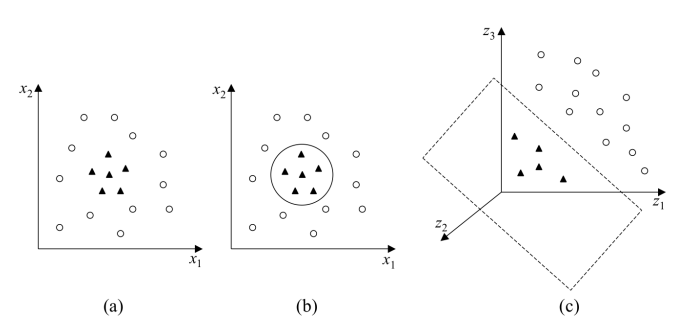
\includegraphics[width=0.7\textwidth, height=3.6cm, keepaspectratio=false]{Imagens/svm_nao_linear.png}
  \end{figure}
\end{frame}

\begin{frame}{Validação Cruzada: Leave-One-Out (LOOCV)}
   Com amostras pequenas, dividir os dados em treino e teste fixos atrapalha os algoritmos e causa erros ou sobreajuste, sendo melhor usar a validação cruzada \textit{Leave-One-Out} (LOOCV) para obter um resultado estável.
  \[
    E_{\mathrm{LOO}} = \frac{1}{n}\sum_{i=1}^n \mathbb{I}\left(g^{\backslash i}(x_i) \neq y_i\right)
  \]
  \begin{itemize}
    \item Necessária pelo tamanho amostral restrito ($n=14$);
    \item Estimador quase não-enviesado do erro de generalização (Luntz--Brailovsky);
    \item Padronização e PCA ajustados \textbf{exclusivamente} sobre o conjunto de treino em cada iteração -- sem vazamento de dados.
  \end{itemize}
\end{frame}

% =====================================================================
\section{RMSD como Método de Referência (Baseline)}
% =====================================================================

\begin{frame}{RMSD e o Algoritmo de Kabsch}
  Neste trabalho, o RMSD é usado como métrica base tradicional (distância euclidiana estática) para comparar as formas Apo e Holo da MBP, servindo como referência para avaliar as novas métricas topológicas estudadas.
  \[
    \mathrm{RMSD}(V,W) = \min_{R,\vec t} \sqrt{\frac{1}{N}\sum_{i=1}^N \left\| R v_i + \vec t - w_i \right\|^2}
  \]
  \begin{itemize}
    \item Solução exata via SVD da matriz de covariância (Algoritmo de Kabsch);
    \item Métrica puramente geométrica/estática -- não captura correlações dinâmicas globais;
    \item Sem escala absoluta de interpretação: cutoffs (ex.\ 3~\AA) dependem do comprimento da cadeia (Maiorov \& Crippen);
    \item Usado como método de comparação (baseline) contra o classificador topológico.
  \end{itemize}
\end{frame}

% =====================================================================
\section{Metodologia}
% =====================================================================

\begin{frame}{Aquisição e Preparação dos Dados}
  \begin{itemize}
    \item Conjunto de calibração: 14 estruturas de Kovacev-Nikolic et al. (2016) -- 7 Apo, 7 Holo;
    \item Expansão: mineração de \textbf{29 novas estruturas} de alta resolução no PDB;
    \item Limpeza via \texttt{ProDy}: extração de coordenadas $(x,y,z)$ dos $C_\alpha$ da Cadeia A;
    \item Matrizes espaciais padronizadas $370 \times 3$ por estrutura.
  \end{itemize}
\end{frame}

\begin{frame}{Extração da Dinâmica e Filtração}
  \begin{itemize}
    \item ANM (\texttt{ProDy}) $\to$ 20 primeiros modos normais $\to$ matriz $C$ ($370\times370$);
    \item $D_{ij} = 1-|C_{ij}|$ $\to$ filtração de Vietoris-Rips com $t_{\max}=0.7$;
    \item Escolha de $t_{\max}$: laços de $H_1$ nascem em $t\approx 0.2$ e morrem antes de $t=0.6$.
  \end{itemize}
\end{frame}

\begin{frame}{Extração da Dinâmica e Filtração}
  \begin{figure}[H]
        \centering
        
        % --- PRIMEIRA LINHA (4 imagens) ---
        \begin{minipage}[b]{0.18\textwidth}
            \centering
            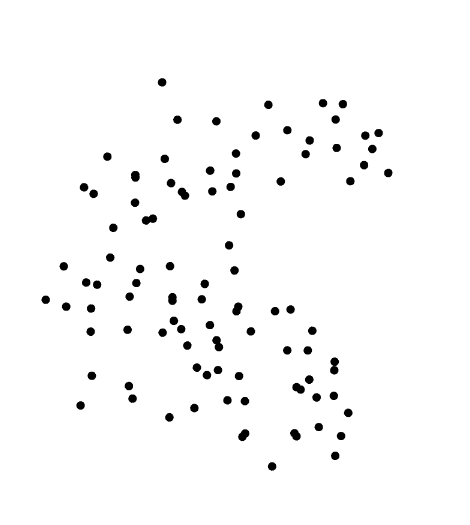
\includegraphics[width=\textwidth]{Imagens/mbp_d1.png}
            {\scriptsize $d = 1.0$Å}
        \end{minipage}\hspace{0.1cm}
        \begin{minipage}[b]{0.18\textwidth}
            \centering
            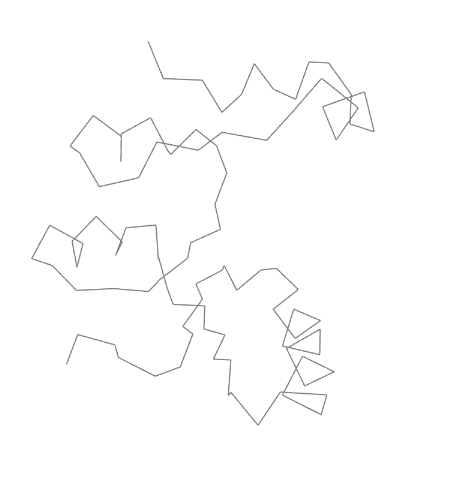
\includegraphics[width=\textwidth]{Imagens/mbp_d4.png}
            {\scriptsize $d = 4.0$Å}
        \end{minipage}\hspace{0.1cm}
        \begin{minipage}[b]{0.18\textwidth}
            \centering
            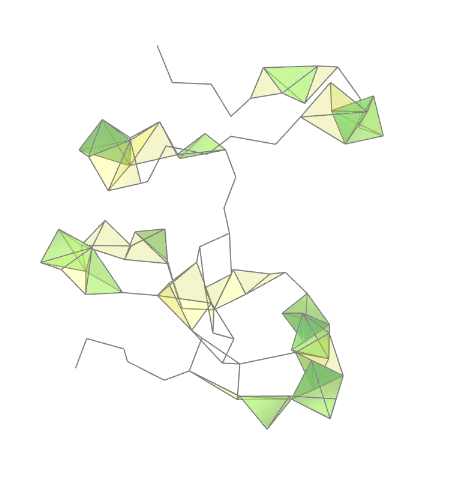
\includegraphics[width=\textwidth]{Imagens/mbp_d55.png}
            {\scriptsize $d = 5.5$Å}
        \end{minipage}\hspace{0.1cm}
        \begin{minipage}[b]{0.18\textwidth}
            \centering
            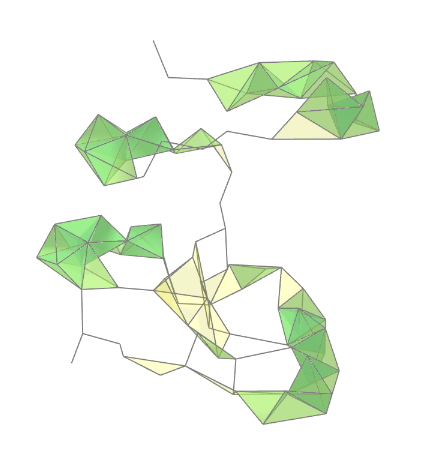
\includegraphics[width=\textwidth]{Imagens/mbp_d6.png}
            {\scriptsize $d = 6.0$Å}
        \end{minipage}
        
        \vspace{0.2cm} % Espaçamento vertical entre as linhas
        
        % --- SEGUNDA LINHA (4 imagens) ---
        \begin{minipage}[b]{0.18\textwidth}
            \centering
            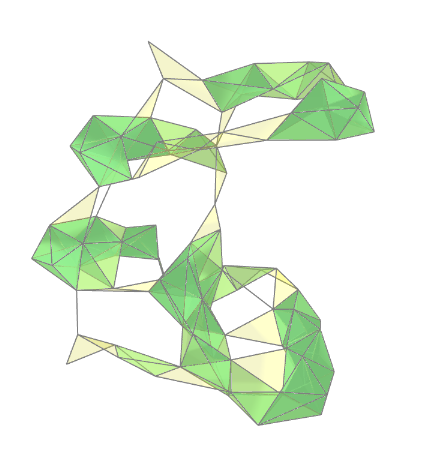
\includegraphics[width=\textwidth]{Imagens/mbp_d7.png}\\[0.1cm]
            {\scriptsize $d = 7.0$Å}
        \end{minipage}\hspace{0.1cm}
        \begin{minipage}[b]{0.18\textwidth}
            \centering
            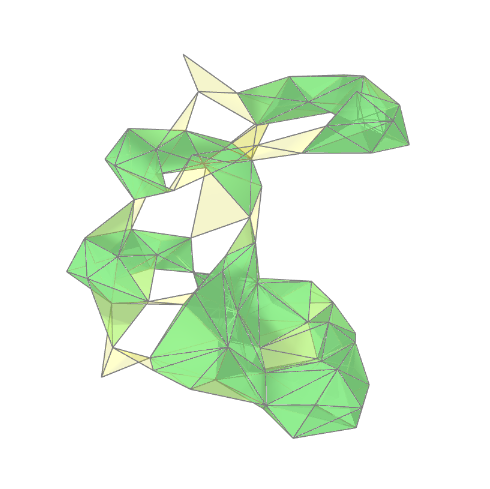
\includegraphics[width=\textwidth]{Imagens/mbp_d8.png}\\[0.1cm]
            {\scriptsize $d = 8.0$Å}
        \end{minipage}\hspace{0.1cm}
        \begin{minipage}[b]{0.18\textwidth}
            \centering
            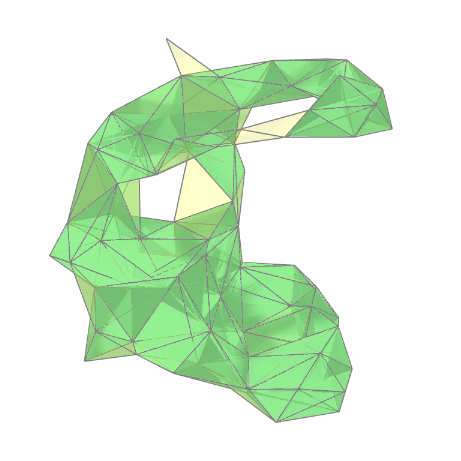
\includegraphics[width=\textwidth]{Imagens/mbp_d9.png}\\[0.1cm]
            {\scriptsize $d = 9.0$Å}
        \end{minipage}\hspace{0.1cm}
        \begin{minipage}[b]{0.18\textwidth}
            \centering
            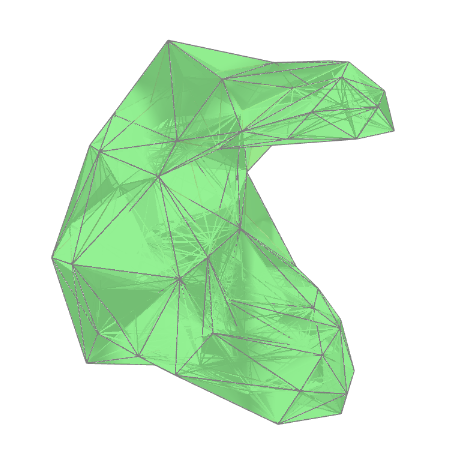
\includegraphics[width=\textwidth]{Imagens/mbp_d12.png}\\[0.1cm]
            {\scriptsize $d = 12.0$Å}
        \end{minipage}     
    \end{figure}
\end{frame}

\begin{frame}{Vetorização e Classificação}
  \begin{itemize}
    \item Paisagem de persistência: $K=73$ camadas $\times$ $R=50$ pontos $\to$ vetor $\mathbb R^{3650}$;
    \item Padronização + PCA (3 componentes principais, $\sim 52{,}5\%$ da variância em $H_1$);
    \item SVM linear ($C=1{,}0$), validado por LOOCV, sem vazamento de dados.
  \end{itemize}

  \begin{figure}[H]
    \centering
    \begin{minipage}[b]{0.48\textwidth}
        \centering
        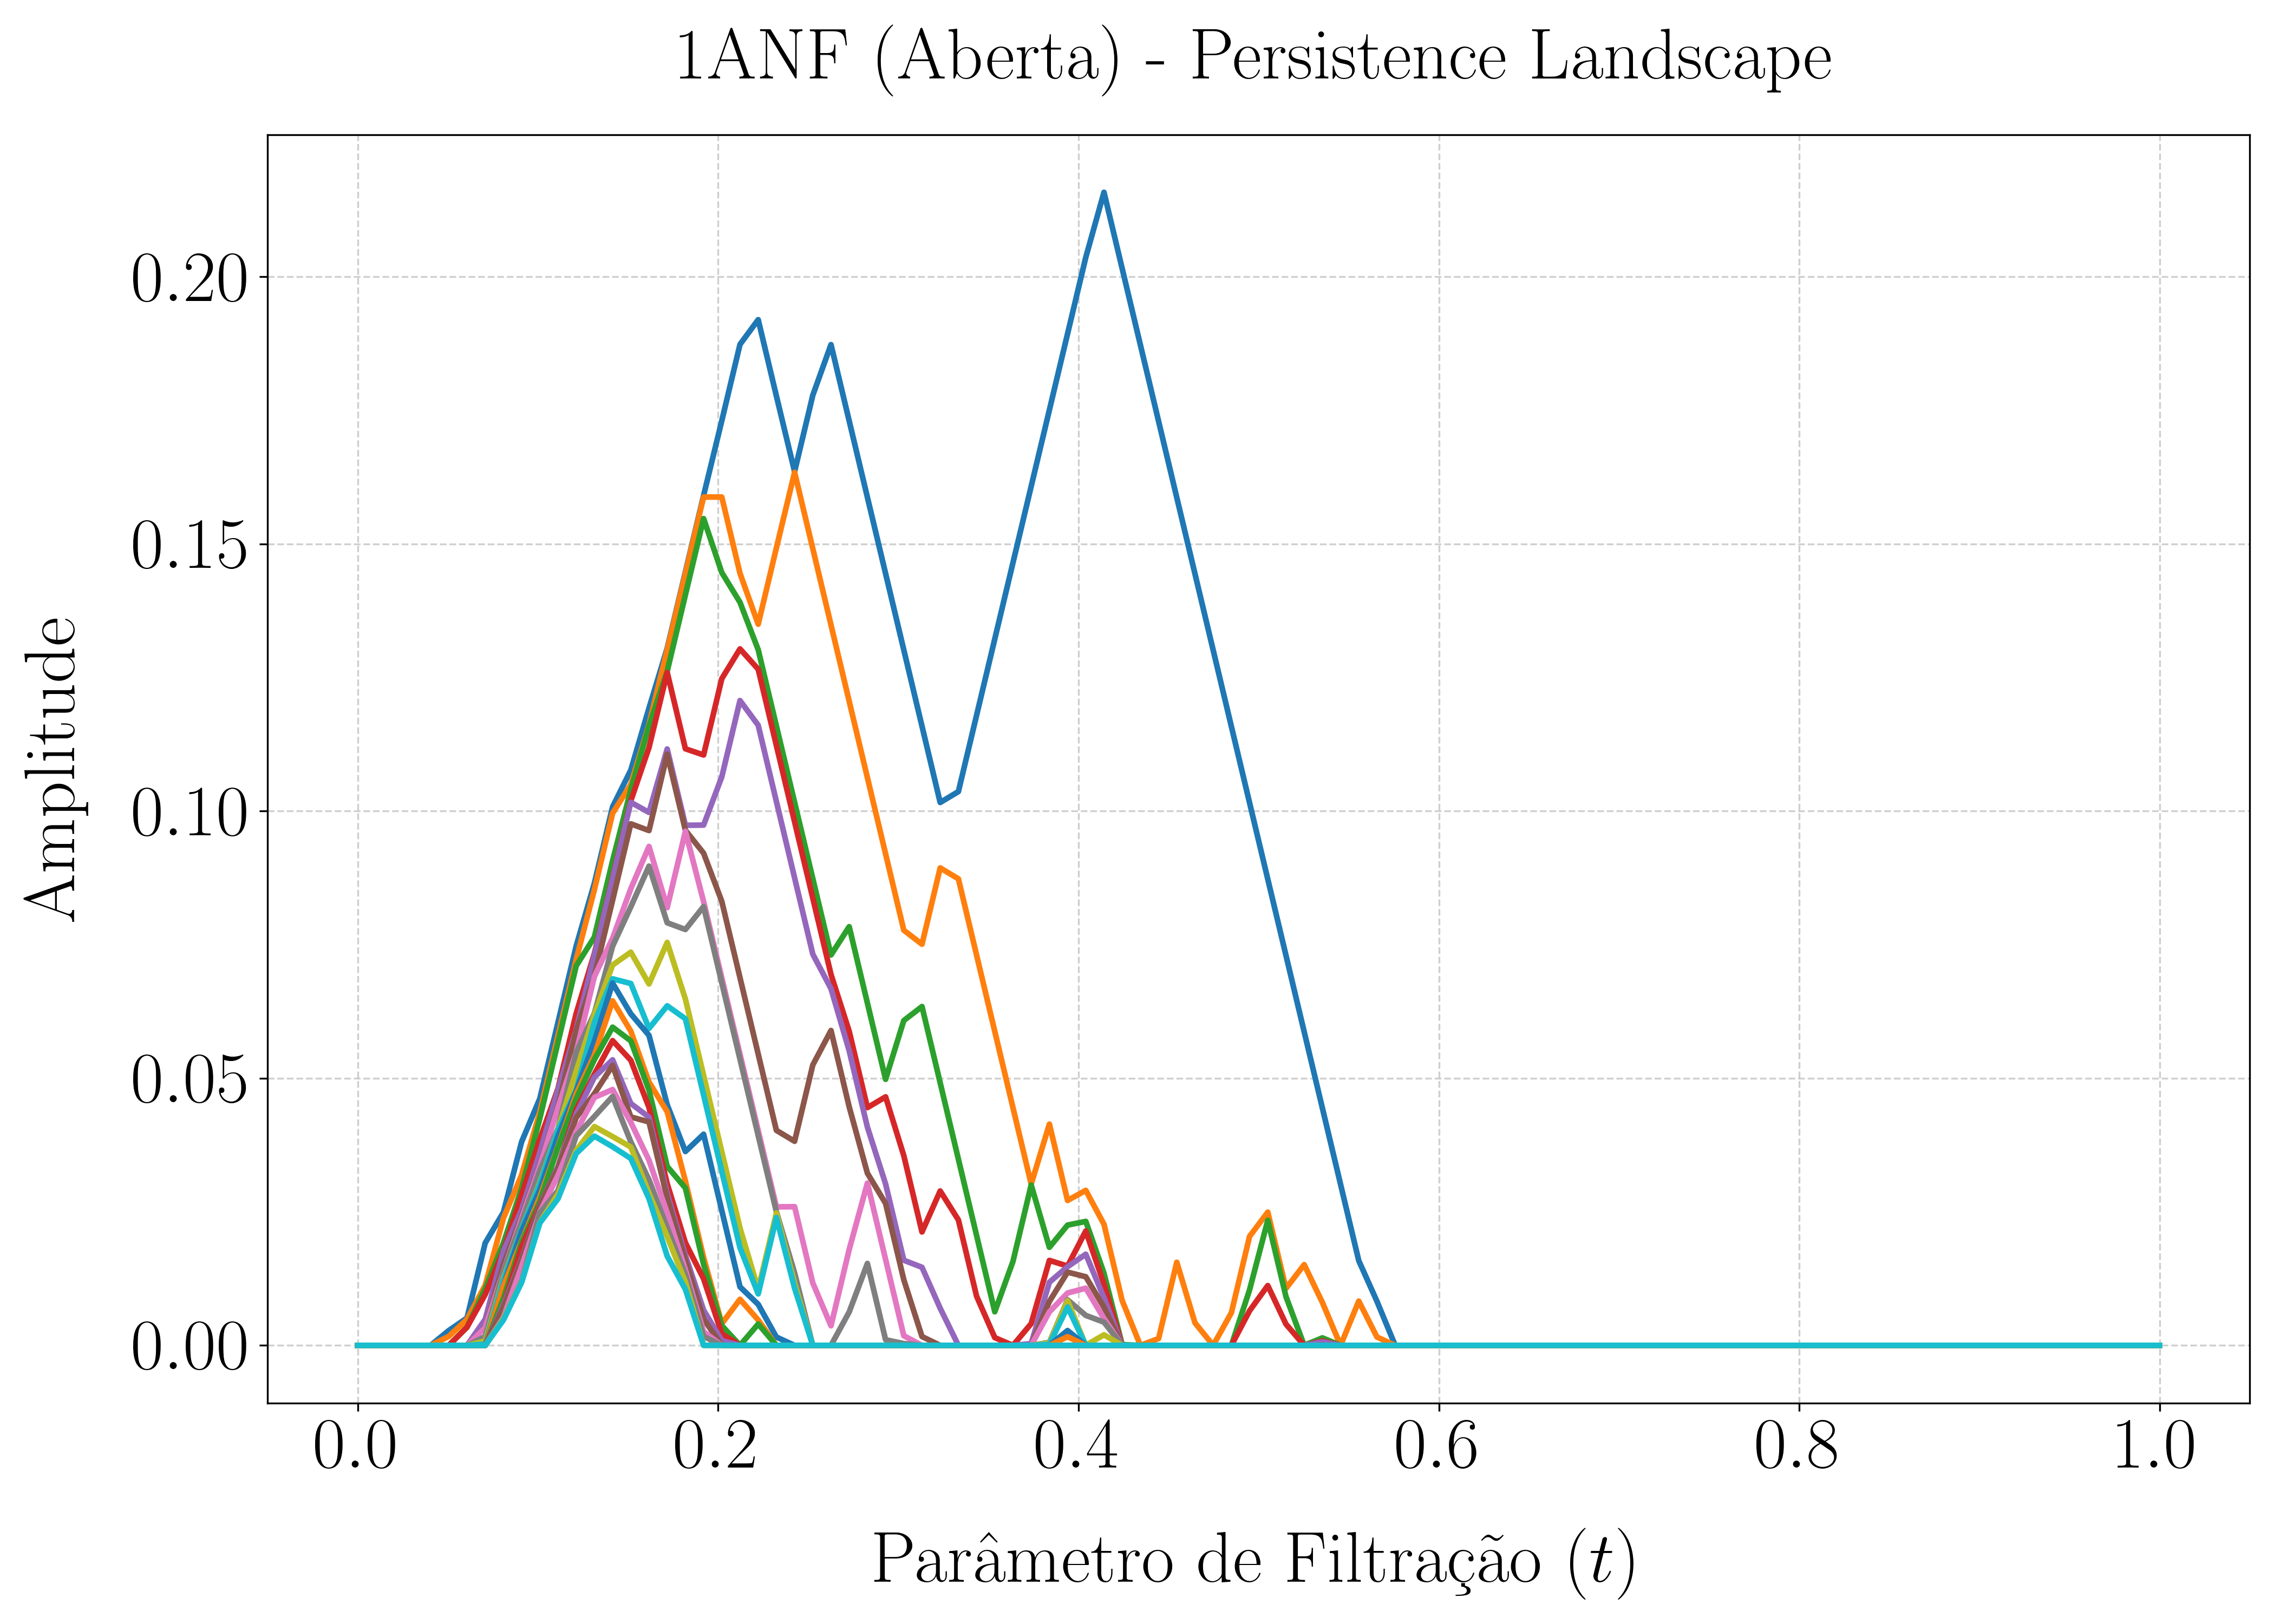
\includegraphics[width=\textwidth]{Imagens/landscape_1ANF.png} 

    \end{minipage}
    \hfill
    \begin{minipage}[b]{0.48\textwidth}
        \centering
        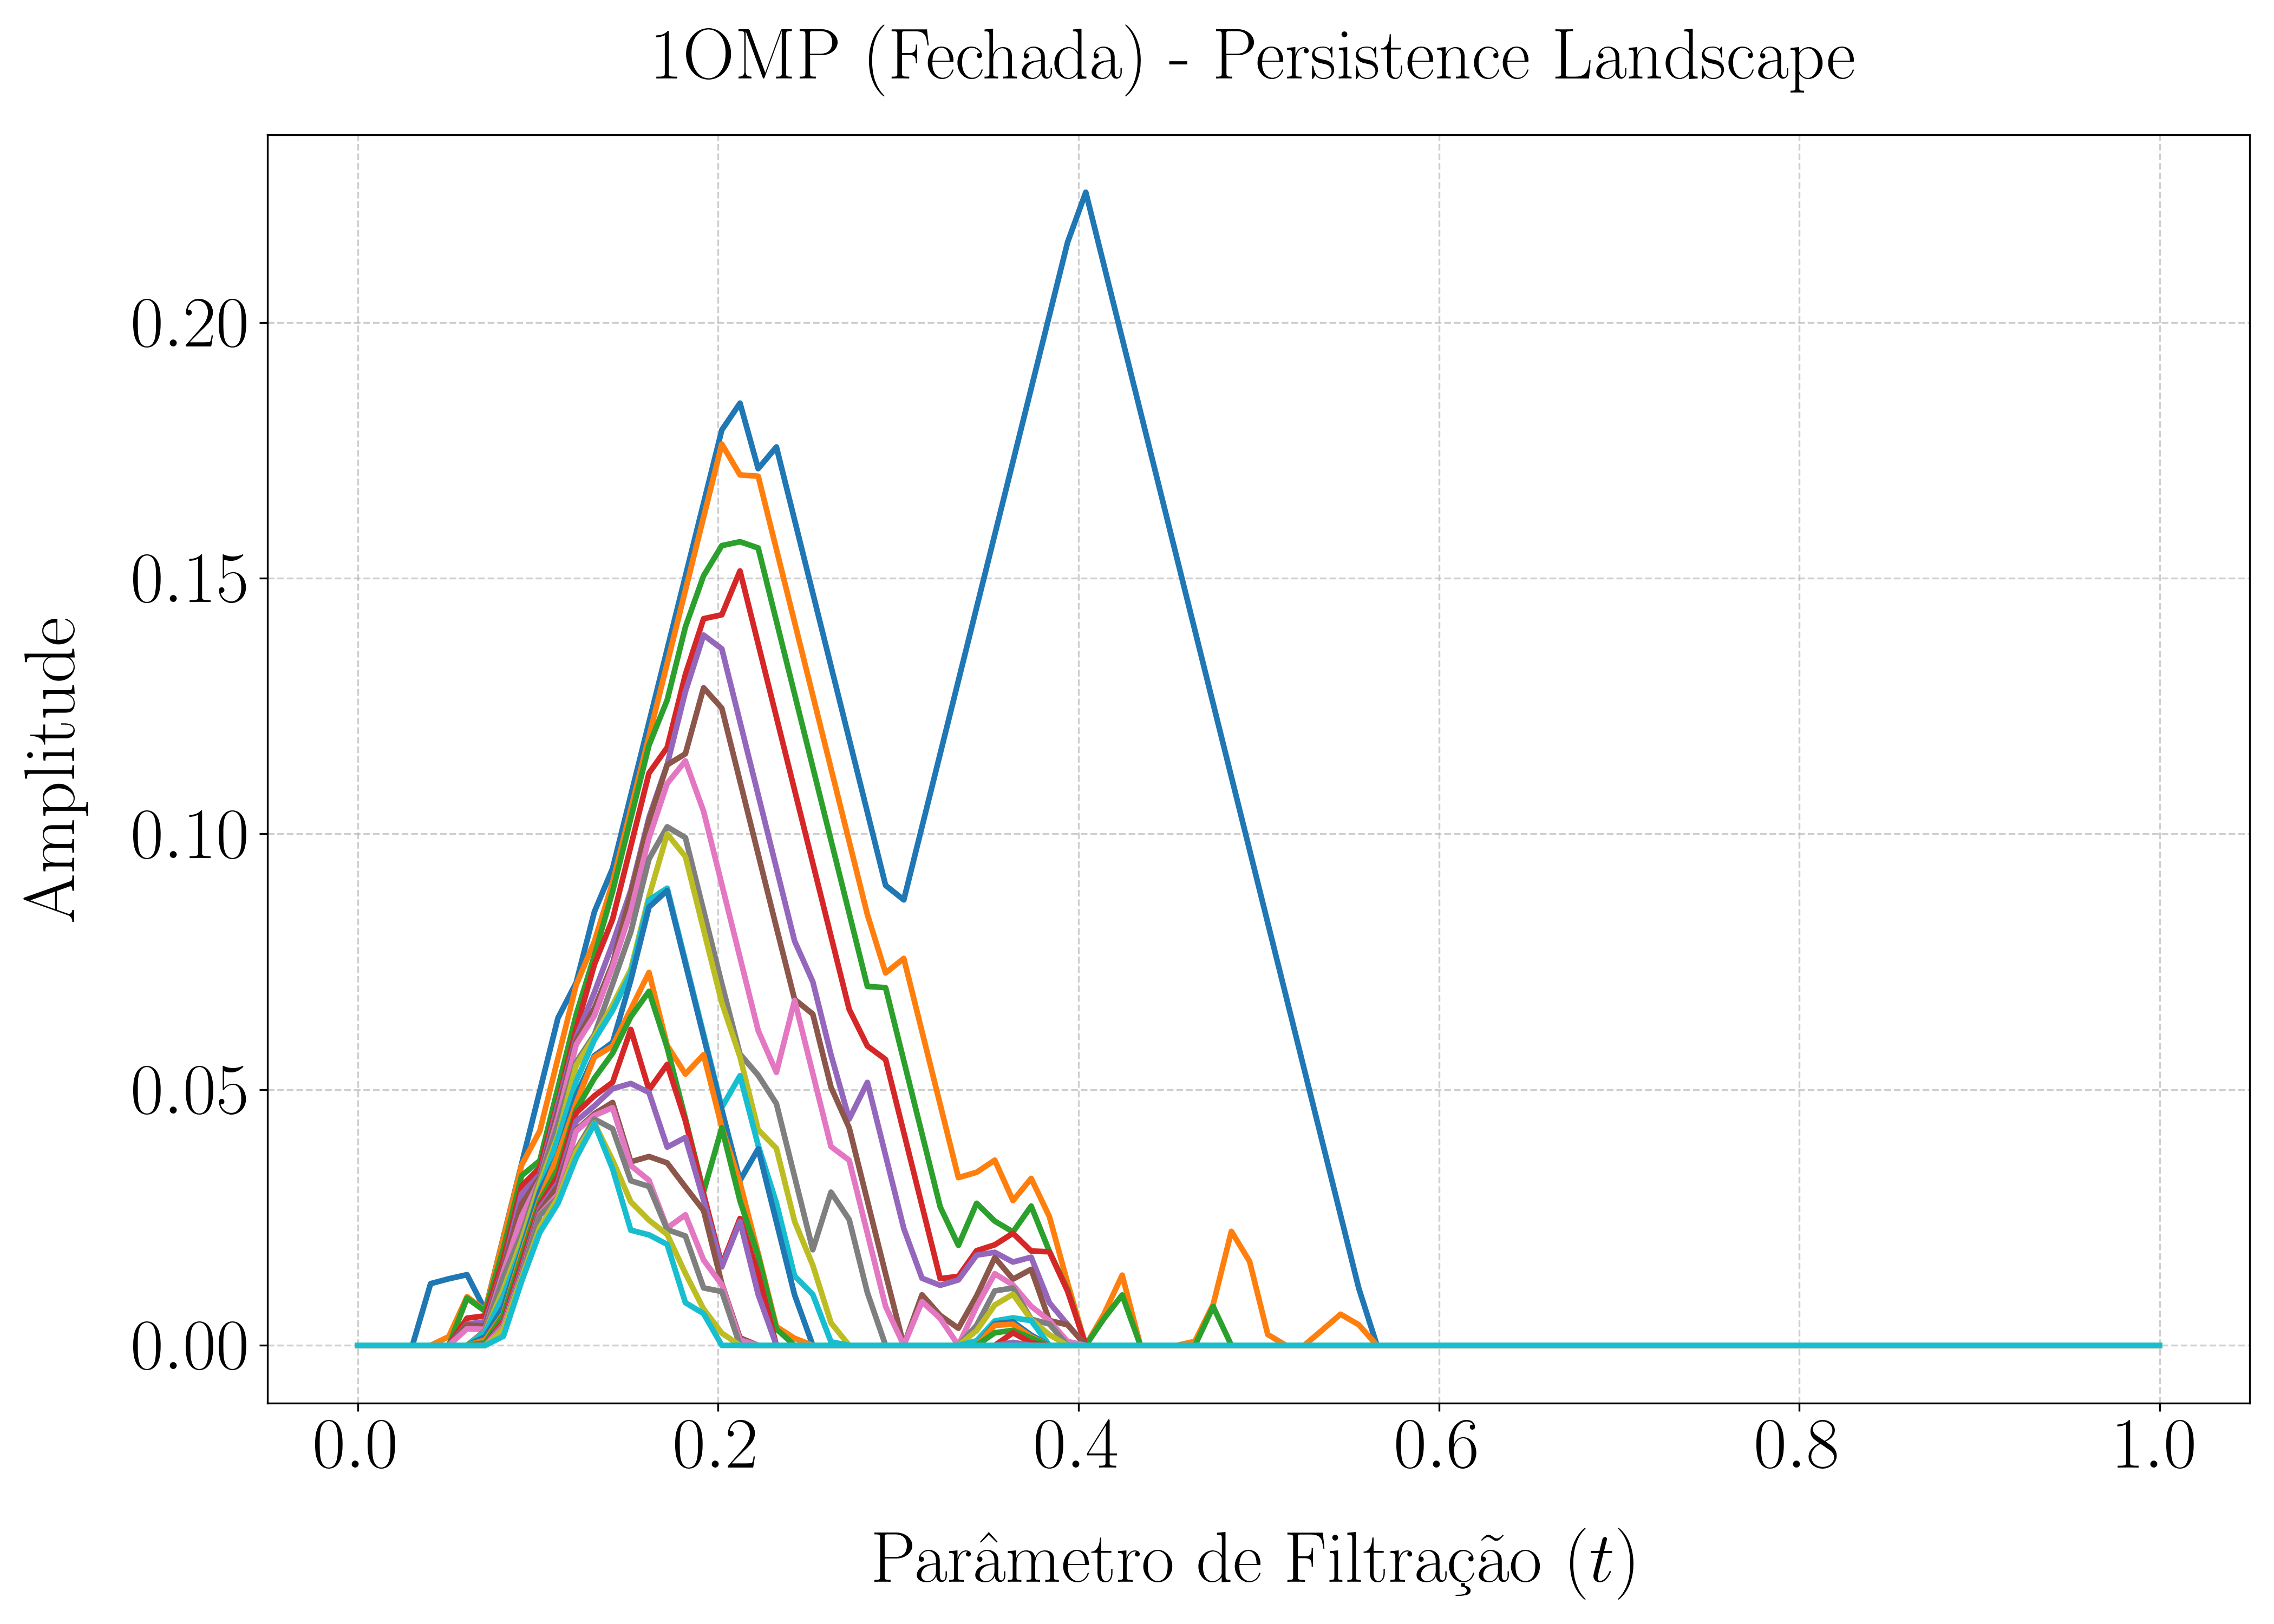
\includegraphics[width=\textwidth]{Imagens/landscape_1OMP.png} 
    \end{minipage}
  \end{figure}
\end{frame}

% =====================================================================
\section{Resultados}
% =====================================================================

\begin{frame}{Teste de Permutação: Resultado}
  \begin{itemize}
    \item $\bar X_{\mathrm{Holo}} = 0{,}269778$, \quad $\bar X_{\mathrm{Apo}} = 0{,}290403$
    \item $T_{\mathrm{obs}} = 0{,}020625$
    \item Das $M=3432$ permutações, apenas $2$ superaram $T_{\mathrm{obs}}$
  \end{itemize}
  \[
    \text{valor-p} = \frac{2}{3432} \approx 5{,}83 \times 10^{-4} \ll \alpha = 0{,}05
  \]
  \textbf{Conclusão:} rejeita-se $H_0$ -- a assinatura topológica das flutuações difere significativamente entre Apo e Holo.
\end{frame}

\begin{frame}{Validação Independente: SVM vs.\ RMSD}
  Avaliação sobre as 29 estruturas mineradas independentemente:
  \begin{table}
    \centering
    \small
    \begin{tabular}{lccccc}
      \toprule
      \textbf{Modelo} & \textbf{Acurácia} & \textbf{Precisão} & \textbf{Sensibilidade} & \textbf{Especificidade} & \textbf{F1} \\
      \midrule
      SVM Topológico & 93{,}10\% & 91{,}67\% & 91{,}67\% & 94{,}12\% & 91{,}67\% \\
      RMSD Médio (baseline) & 89{,}66\% & 84{,}62\% & 91{,}67\% & 88{,}24\% & 88{,}00\% \\
      \bottomrule
    \end{tabular}
  \end{table}
  \begin{itemize}
    \item Mesmo número de falsos negativos (1DMB, em ambos);
    \item SVM: menos falsos positivos (1 vs.\ 2);
    \item Diferença pontual (29 amostras) -- sem teste de McNemar formal.
  \end{itemize}
\end{frame}

\begin{frame}{Projeção do Hiperplano de Decisão}
  \begin{figure}
    \centering
    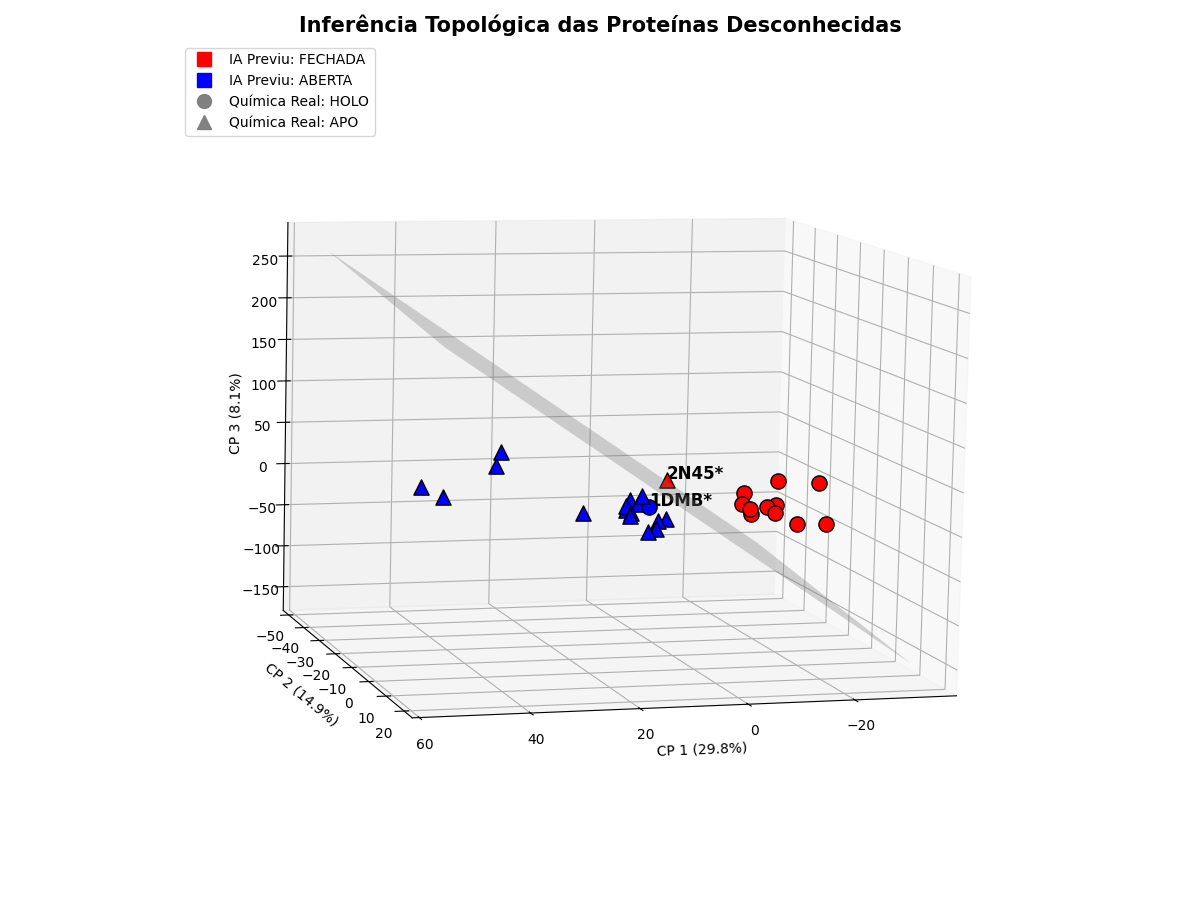
\includegraphics[width=0.75\textwidth]{Imagens/svm_proteinas.png}
  \end{figure}
\end{frame}

\begin{frame}{Robustez Topológica contra Artefatos de Alinhamento}
  \textbf{Caso 7Z7H:} RMSD $> 26$~\AA\ (erro catastrófico).
  \begin{itemize}
    \item Causa: \textit{gaps} de numeração na cadeia (mismatch de índices);
    \item RMSD exige correspondência estrita de índices $\to$ colapsa;
    \item SVM topológico opera sobre a matriz \textbf{intrínseca} de conectividade (ANM) $\to$ invariante a artefatos de numeração;
    \item Classificação correta (``Aberta'') mantida pelo método topológico.
  \end{itemize}
\end{frame}

\begin{frame}{Assinaturas Dinâmicas e Seleção Conformacional}
  \begin{itemize}
    \item \textbf{1DMB} (rotulada Holo): classificada como Aberta por \emph{ambos} os métodos -- possível falha de cristalização do ligante.
    \item \textbf{2N45} (rotulada Apo): RMSD $\to$ Aberta; SVM $\to$ Fechada, com baixa confiança (distância ao hiperplano $d=0{,}1985$).
    \item Resultado limítrofe compatível com a hipótese de \textbf{Seleção Conformacional}: o método topológico capta estados transientes de flexibilidade latente.
  \end{itemize}
\end{frame}

% =====================================================================
\section{Conclusão}
% =====================================================================

\begin{frame}{Conclusão}
  \begin{itemize}
    \item A transformação $D_{ij}=1-|C_{ij}|$ traduz a dinâmica do ANM em um espaço de dissimilaridade apto à TDA;
    \item A Homologia Persistente e as Paisagens de Persistência fornecem uma base rigorosa (espaço de Hilbert) para a classificação estatística e via SVM;
    \item O teste de permutação confirma separabilidade estatística significativa ($p \approx 5{,}83\times10^{-4}$);
    \item O classificador topológico superou o RMSD clássico, com maior robustez frente a artefatos estruturais;
    \item Evidências compatíveis com o modelo biológico de Seleção Conformacional.
  \end{itemize}
\end{frame}

\begin{frame}{Agradecimentos}
  \centering
  \begin{center}
    {\Huge \textbf{Obrigado!}}
  \end{center}
  \vfill
  \begin{block}{}
    \centering
    \vspace{0.2cm}
    \large \itshape ``É justo que muito me custe o que muito me vale.'' \\[0.3cm]
    \small \upshape --- Santa Teresa d'Ávila
    \vspace{0.2cm}
  \end{block}

  \vfill
  {\centering \rule{0.5\textwidth}{0.4pt}\par} % Linha horizontal centralizada
  \vfill

  \begin{center}
    \small
    \textbf{Anthony dos Anjos Marques} \\
    \textbf{Orientador:} Prof. Dr. Danilo Dias da Silva \\
    \footnotesize Departamento de Matemática -- UFS
  \end{center}
  % \small Anthony dos Anjos Marques \\
  % Orientador: Prof. Dr. Danilo Dias da Silva \\
  % Departamento de Matemática -- UFS
\end{frame}

\end{document}